\documentclass[preprint, 3p, authoryear]{elsarticle} %review=doublespace preprint=single 5p=2 column
%%% Begin My package additions %%%%%%%%%%%%%%%%%%%

\usepackage[hyphens]{url}

  \journal{Oikos; Article} % Sets Journal name

\usepackage{graphicx}
%%%%%%%%%%%%%%%% end my additions to header

\usepackage[T1]{fontenc}
\usepackage{lmodern}
\usepackage{amssymb,amsmath}
% TODO: Currently lineno needs to be loaded after amsmath because of conflict
% https://github.com/latex-lineno/lineno/issues/5
\usepackage{lineno} % add
\usepackage{ifxetex,ifluatex}
\usepackage{fixltx2e} % provides \textsubscript
% use upquote if available, for straight quotes in verbatim environments
\IfFileExists{upquote.sty}{\usepackage{upquote}}{}
\ifnum 0\ifxetex 1\fi\ifluatex 1\fi=0 % if pdftex
  \usepackage[utf8]{inputenc}
\else % if luatex or xelatex
  \usepackage{fontspec}
  \ifxetex
    \usepackage{xltxtra,xunicode}
  \fi
  \defaultfontfeatures{Mapping=tex-text,Scale=MatchLowercase}
  \newcommand{\euro}{€}
\fi
% use microtype if available
\IfFileExists{microtype.sty}{\usepackage{microtype}}{}

\ifxetex
  \usepackage[setpagesize=false, % page size defined by xetex
              unicode=false, % unicode breaks when used with xetex
              xetex]{hyperref}
\else
  \usepackage[unicode=true]{hyperref}
\fi
\hypersetup{breaklinks=true,
            bookmarks=true,
            pdfauthor={},
            pdftitle={Spatial variation in predator diel activity patterns},
            colorlinks=false,
            urlcolor=blue,
            linkcolor=magenta,
            pdfborder={0 0 0}}

\setcounter{secnumdepth}{5}
% Pandoc toggle for numbering sections (defaults to be off)


% tightlist command for lists without linebreak
\providecommand{\tightlist}{%
  \setlength{\itemsep}{0pt}\setlength{\parskip}{0pt}}

% From pandoc table feature
\usepackage{longtable,booktabs,array}
\usepackage{calc} % for calculating minipage widths
% Correct order of tables after \paragraph or \subparagraph
\usepackage{etoolbox}
\makeatletter
\patchcmd\longtable{\par}{\if@noskipsec\mbox{}\fi\par}{}{}
\makeatother
% Allow footnotes in longtable head/foot
\IfFileExists{footnotehyper.sty}{\usepackage{footnotehyper}}{\usepackage{footnote}}
\makesavenoteenv{longtable}

% Pandoc citation processing
\newlength{\cslhangindent}
\setlength{\cslhangindent}{1.5em}
\newlength{\csllabelwidth}
\setlength{\csllabelwidth}{3em}
\newlength{\cslentryspacingunit} % times entry-spacing
\setlength{\cslentryspacingunit}{\parskip}
% for Pandoc 2.8 to 2.10.1
\newenvironment{cslreferences}%
  {}%
  {\par}
% For Pandoc 2.11+
\newenvironment{CSLReferences}[2] % #1 hanging-ident, #2 entry spacing
 {% don't indent paragraphs
  \setlength{\parindent}{0pt}
  % turn on hanging indent if param 1 is 1
  \ifodd #1
  \let\oldpar\par
  \def\par{\hangindent=\cslhangindent\oldpar}
  \fi
  % set entry spacing
  \setlength{\parskip}{#2\cslentryspacingunit}
 }%
 {}
\usepackage{calc}
\newcommand{\CSLBlock}[1]{#1\hfill\break}
\newcommand{\CSLLeftMargin}[1]{\parbox[t]{\csllabelwidth}{#1}}
\newcommand{\CSLRightInline}[1]{\parbox[t]{\linewidth - \csllabelwidth}{#1}\break}
\newcommand{\CSLIndent}[1]{\hspace{\cslhangindent}#1}


\usepackage{setspace}\doublespacing
\usepackage{lineno}
\usepackage{float}
\floatplacement{figure}{H}
\newcommand{\beginsupplement}{\setcounter{table}{0}  \renewcommand{\thetable}{S\arabic{table}} \setcounter{figure}{0} \renewcommand{\thefigure}{S\arabic{figure}} \setcounter{section}{0} \renewcommand{\thesection}{S\arabic{section}}}
\usepackage{pdflscape}
\newcommand{\blandscape}{\begin{landscape}}
\newcommand{\elandscape}{\end{landscape}}
\usepackage{booktabs}
\usepackage{longtable}
\usepackage{array}
\usepackage{multirow}
\usepackage{wrapfig}
\usepackage{float}
\usepackage{colortbl}
\usepackage{pdflscape}
\usepackage{tabu}
\usepackage{threeparttable}
\usepackage{threeparttablex}
\usepackage[normalem]{ulem}
\usepackage{makecell}
\usepackage{xcolor}



\begin{document}


\begin{frontmatter}

  \title{Spatial variation in predator diel activity patterns}
    \author[UOM,CSIRO]{Matthew W. Rees%
  \corref{cor1}%
  }
   \ead{matt.wayne.rees@gmail.com} 
    \author[UOM]{Brendan A. Wintle%
  %
  }
  
    \author[UOM,CEC]{Jack H. Pascoe%
  %
  }
  
    \author[UOM,CEC]{Mark Le Pla%
  %
  }
  
    \author[CEC]{Emma K. Birnbaum%
  %
  }
  
    \author[UOM]{Bronwyn A. Hradsky%
  %
  }
  
      \affiliation[UOM]{Quantitative and Applied Ecology Group, School of Ecosystem and Forest Sciences, The University of Melbourne, Parkville, VIC, 3010, Australia}
    \affiliation[CSIRO]{Health and Biosecurity, Commonwealth Scientific and Industrial Research Organisation, Ecosciences Precinct, Dutton Park, QLD, Australia}
    \affiliation[CEC]{Conservation Ecology Centre, Lighthouse Rd, Cape Otway, VIC, 3233, Australia}
    \cortext[cor1]{Corresponding author}
  
  \begin{abstract}
  \emph{Open research:} Data and code will be deposited on Dryad upon acceptance and can currently be found at this link: https://github.com/matt-w-rees/spatiotemporal-gams-invasive-predators.
  \end{abstract}
    \begin{keyword}
    diel activity patterns \sep generalised additive model \sep feral cat \sep invasive predator \sep intraguild predator interactions \sep lethal predator control \sep mesopredator release \sep red fox \sep 
    spatiotemporal model
  \end{keyword}
  
 \end{frontmatter}

\parskip=12pt 
\newpage
\setcounter{page}{1}

\hypertarget{spatial-variation-in-predator-diel-activity-patterns}{%
\section*{Spatial variation in predator diel activity patterns}\label{spatial-variation-in-predator-diel-activity-patterns}}
\addcontentsline{toc}{section}{Spatial variation in predator diel activity patterns}

\(~\)

\linenumbers

\hypertarget{abstract}{%
\section*{ABSTRACT}\label{abstract}}
\addcontentsline{toc}{section}{ABSTRACT}

Understanding the constraints dominant predators impose on subordinate species is important for predicting ecosystem dynamics and anticipating outcomes of predator management. Subordinate predators may avoid dominant predators in time or space, making it difficult to quantify antipredator behaviours unless joint spatiotemporal analyses are used.
Here, we tested whether an invasive dominant predator (red fox \emph{Vulpes vulpes}) alters the spatiotemporal activity of an invasive subordinate predator (feral cat \emph{Felis catus}). We collated records of both species from 3,667 camera-traps deployed experimentally across two regions of south-eastern Australia with simplified predator guilds; foxes were poison-baited in some landscapes within each region. We used generalised additive models to quantify changes in predator spatiotemporal activity across geographic space, vegetation types, human footprint and (artificially manipulated) gradients of dominant predator activity.
Foxes and cats had similar diel activity patterns when averaged across all sites, however there was important differentiation at a finer scale---cats did not reduce their spatial activity but shifted diel patterns when localised fox activity was high. Cats were crepuscular on average. However, across dry vegetation types of both regions (where foxes were nocturnal), cats shifted to diurnal behaviour with increasing fox activity. In contrast, fox activity was relatively consistent throughout the daily cycle in the wet forest; here cats avoided dawn when fox activity was high. Changes in cat diel activity patterns may facilitate spatial coexistence between these two invasive predators, potentially shifting feral cat impacts onto different native prey.
It is well-appreciated that predator activity varies spatially and fluctuates throughout the daily cycle. However, our study demonstrates that diel activity patterns also vary across space, likely mediated by both landscape-context and fear. dominant predator avoidance appears to be dynamic---a key nuance which is overlooked when simply comparing the average activity overlap between two species.

\newpage

\hypertarget{introduction}{%
\section{INTRODUCTION}\label{introduction}}

Top predators can drive ecosystem structure and dynamics by suppressing populations of rival predators and prey species (Prugh et al. 2009, Estes et al. 2011). Dominant predators can suppress subordinate species directly through antagonistic interactions and predation, as well as indirectly through fear (Creel and Christianson 2008, Allen et al. 2022). Fear-induced behavioural suppression can be as detrimental to subordinate species as predation itself, by limiting resource acquisition and breeding success (Brown et al. 1999, Schmitz et al. 2004, Preisser et al. 2005). Understanding how top predators---including humans---constrain the behaviour of subordinate species is therefore important to accurately predict consequences of predator management, such as reintroductions or lethal control (Suraci et al. 2016, Gaynor et al. 2021).

Spatial and/or temporal niche partitioning may allow subordinate species to coexist with top predators by reducing encounter-rates and resource overlap (Kronfeld-Schor and Dayan 2003). However, subordinate species may not consistently employ avoidance behaviours because perceived predation risk is spatiotemporally variable, and antipredator behaviours typically involve a trade-off against resource acquisition, such as limiting or relegating activity to suboptimal places or times (Lima and Dill 1990, Lima and Bednekoff 1999). Therefore, optimal predator avoidance strategies likely vary across heterogeneous landscapes where resource availability (e.g., shelter, food) and perceived predation risks differ (Kauffman et al. 2007, Willems and Hill 2009, Davies et al. 2021, Wirsing et al. 2021). For example, temporal predator avoidance may be preferable over spatial avoidance if food is constantly available throughout the day, and vice versa. These theories are unified under the ecology of fear concept (Brown et al. 1999), which has gained increasing attention in recent times (Gaynor et al. 2019). However, there remains a lack of robust, empirical evidence documenting dynamic changes in antipredator behaviour.

Animal diel activity patterns are increasingly being considered alongside spatial activity and distributional patterns. However, spatial and temporal (in regard to the daily cycle) activity patterns are still often considered in an ad-hoc fashion. For example, by fitting separate models for spatial and temporal overlap, or by repeating spatial analyses (e.g., resource selection functions) at different time periods such night and day (e.g., Basille et al. 2015, Kohl et al. 2019, Smith et al. 2019, Wooster et al. 2022). Such ad-hoc approaches make it difficult to assess the relative importance, as well as dynamic changes in spatial and temporal processes (Suraci et al. 2022).

There are many approaches to modelling intraguild spatiotemporal interactions, such as time-to-encounter models and coefficients of activity overlap (Frey et al. 2017). Time-to-encounter approaches consider fine-scale avoidance or attraction by using time intervals between species detections as the response variable, although do not estimate diel activity patterns (Harmsen et al. 2009, Fancourt et al. 2019, Niedballa et al. 2019). Multispecies models have been recently developed to assess overlap in spatial and diel activity between two species (Ait Kaci Azzou et al. 2021), as well as different diel activity patterns based on the presence or absence of another species at a site (Kellner et al. 2022). Multispecies models are data-hungry and difficult to fit, but can account for imperfect detection and different types of predictor variables (e.g., Parsons et al. 2022). Given avoidance behaviours are likely dynamic (Gaynor et al. 2019), there is need for statistical approaches which jointly assess continuous shifts in spatial and diel activity patterns of one species in response to another, particularly when combined with experimental data (Suraci et al. 2022).

Generalised Additive Models (hereafter `GAMs') are increasingly being used to estimate animal diel activity patterns and offer a flexible framework to jointly consider spatial activity. GAMs are useful to model diel activity patterns as they can implement cyclical splines---joining the end with the start of the day---as well as complexity penalties to reduce overfitting. If complex nonlinear (i.e., wiggly) effects are not statistically supported, smoothing penalties in GAMs `shrink' them to a linear (i.e., no wiggliness) effect, or even to a horizontal line - removing the entire effect of the predictor variable and therefore the need for additional tests of statistical significance (such as p-values and information criteria). GAMS can also capture nonlinear interactions between multiple variables with different units (i.e., `tensor products'), and offer the ability to share information across categorical variables through hierarchical specifications (Wood 2017, Pedersen et al. 2019). However, we are only aware of one study which allowed animal diel activity to interact with predation risk as a continuous variable in a GAM (although without considering overall activity, Cunningham et al. 2019).

The red fox \emph{Vulpes vulpes} (hereafter `fox') and feral cat \emph{Felis catus} (hereafter `cat') have devastating impacts on native prey throughout their introduced range, implicated in the extinction of \textasciitilde10 and 63 species, respectively (Doherty et al. 2016). The impacts of these invasive predators are particularly extreme on the Australian continent (Woinarski et al. 2015). Cats are more difficult to manage, and so introduced predator control programs in Australia often target only foxes (particularly through poison-baiting, Reddiex et al. 2007). As foxes and cats compete for many of the same resources (Fleming et al. 2022), there is concern that lethal fox control could cause mesopredator release (Soulé et al. 1988) of cats (Glen and Dickman 2005, Doherty and Ritchie 2017, Wayne et al. 2017). However, there is limited evidence that spatial cat activity increases in response to fox control (Hunter et al. 2018), although there are signs of changes in behaviour and population density (Molsher et al. 2017, Rees et al. 2023a). Other studies have investigated potential spatial and temporal interactions between these invasive predators (e.g., Roshier and Carter 2021), but not in response to fox control, or in a joint spatiotemporal framework that allows flexibility in cat avoidance behaviours with respect to differences in fox activity. Conservation managers are therefore uncertain as to whether fox control may increase the impacts of feral cats on native prey, through increases in cat density or behavioural changes which improve hunting success.

In this study, we first explored (1) how predator diel activity patterns vary across geographic space (`model 1'), and (2) the role of vegetation type and human footprint in predator activity patterns (`model 2'). Using this knowledge to partition our dataset, we then (3) tested whether the activity of a dominant predator (fox) affected the spatiotemporal activity of a subordinate predator (cat; `model 3'). In line with behavioural avoidance or exclusion, we predicted that cat diel activity pattens would shift towards less-risky times of day (i.e., times when fox activity was lower), and/or spatial cat activity would be lower at sites where fox activity was relatively high. We illustrate how GAMs can provide a simple framework to jointly assess spatial and temporal animal activity patterns, as well as potential species interactions.

\newpage

\hypertarget{materials-and-methods}{%
\section{MATERIALS AND METHODS}\label{materials-and-methods}}

\hypertarget{study-area-and-camera-trapping}{%
\subsection{Study area and camera-trapping}\label{study-area-and-camera-trapping}}

Our study was conducted in a simple predator system where foxes and cats are the only medium-large (\textgreater{} 1 kg) mammalian predators, and fox activity is manipulated using lethal control in some landscapes. This situation allowed sole focus on the interactions between these two predators, across an experimental gradient of dominant predator (fox) activity. We compiled data from multiple smaller-scale camera-trap studies, each designed to experimentally assess mammal responses to fox control. Overall, we collated 5,449 and 2,202 independent detections of foxes and cats, respectively (separated by at least 30 minutes) from 172,052 camera-trap nights (Table \ref{tab:diel-tab1}).

We collated camera-trap data across two regions in south-west Victoria, Australia: the Glenelg region and Otway Ranges (Fig. \ref{fig:diel-map}). Here, dingoes \emph{Canis familiaris} are long-absent throughout, while tiger quolls \emph{Dasyurus maculatus} are long-absent in the Glenelg region and likely functionally extinct in the Otway Ranges (last confirmed sighting in 2014). In broad sections of each region, government land managers conduct ongoing targeted lethal fox control for biodiversity conservation (see sections below for region-specific details). Poison-baits containing 3 mg of sodium fluroacetate (compound 1080) are buried at a depth of 12 - 15 cm at 1-km intervals along accessible forest tracks and roads. Different road densities therefore result in variable densities of poison-baits. Foxes readily dig these poison-baits often resulting in population suppression, whereas it is generally accepted that cats are unlikely to consume buried fox-baits and there is no evidence buried 1080 fox-baits suppresses cat populations (Risbey et al. 1997, Algar and Burrows 2004, Moseby et al. 2011, Hunter et al. 2018). Managers also frequently implement prescribed fire across both regions, primarily to reduce fuel loads to prevent large wildfires.

\hypertarget{glenelg-region}{%
\subsubsection{Glenelg region}\label{glenelg-region}}

In the Glenelg region, large patches of natural vegetation are fragmented by pastoral farming and residential properties (Fig. \ref{fig:diel-map}). Foxes in three distinct forest blocks in this region have been subject to poison-baiting since October 2005, with fortnightly bait replacements (Robley et al. 2014). These forest blocks, along with three similar, unbaited forest blocks to the north have been simultaneously surveyed annually under the `Glenelg Ark' fox control program since 2005 (40 sites per block, Robley et al. 2020). Hair-tubes were used to monitor species from 2005 - 2013 (presented in Robley et al. 2014), replaced by camera-traps from 2013; here we present camera-trap data from 2013 - 2019 (Robley et al. 2020). We also included a further 425 camera-trap deployments at unique locations from early 2018 (M.W.R PhD Surveys', Rees et al. 2023b). This totals 2,039 camera-trap deployments in the Glenelg region, collected in a control-impact experimental design (foxes had been continuously controlled for at 8 - 14 years in the treatment landscapes at the time of these surveys).

\hypertarget{otway-ranges}{%
\subsubsection{Otway Ranges}\label{otway-ranges}}

The Otway Ranges is a largely continuous patch of natural vegetation with a strong east-west rainfall gradient (Fig. \ref{fig:diel-map}). A matrix of cool temperate rainforest and wet forest at high altitudes in the south-west descend into a large heathland directly north, and into dry forests and then heathlands to the north-east. Fox-baiting commenced in small sections of the Otway Ranges in 2008 and large-scale systematic baiting began in 2016 - 2017 under the `Otway Ark' program (Robley et al. 2019). For the first six weeks, poison-baits were replaced weekly, then changing to ongoing monthly bait-replacement. There was a pause in baiting for approximately six months during the second half of 2018. Fox control recommenced in late 2018 with four weeks of fortnightly bait-replacement, before returning to monthly bait-replacement. A large section of the Otway Ranges to the north-west remains unbaited, but is monitored as an experimental non-treatment site (Robley et al. 2019). Otway Ark managers survey 372 camera-trap sites annually (sequentially across the region); we present one `before' baiting survey and two `after' baiting surveys of each site from 2016 - 2018, totalling 1,113 camera-trap deployments (Robley et al. 2019). We also include data from an additional before-after control-impact surveys (one `before' baiting survey and two `after' baiting surveys) in the western section of the Otway Ranges, conducted annually 2017 - 2019 (Rees et al. 2023b). This added a further 195 sites and 524 camera-trap deployments (Table \ref{tab:tab-sum}).

\hypertarget{camera-trap-set-ups}{%
\subsubsection{Camera-trap set-ups}\label{camera-trap-set-ups}}

All camera-trap deployments consisted of a Reconyx (Holmen, Wisconsin) brand camera-trap (white or infrared flash), attached to a tree or a metal picket, facing a lure. All camera-trap sites were positioned in the forest interior at least 30 m away from roads. The Glenelg Ark and Otway Ark fox monitoring programs positioned camera-traps at least 40 cm above ground on a tree or a metal picket and angled downwards toward a lure approximately 1 - 1.5 m away (Robley et al. 2019, 2020). The lures consisted of peanut butter, golden syrup and rolled oats mixed into a small ball, placed within a tea strainer or PVC pipe container and secured either to the ground, or 20 - 60 cm above ground on a wooden stake. The M.W.R PhD surveys across both regions positioned camera-traps lower on a tree (around 15 - 30 cm above the ground) angled only slightly downwards toward a tuna oil lure approximately 2 - 2.5 m away (detailed in Rees et al. 2023a). Camera-traps were active for an average of 47 days (maximum 93 days), totalling 172,052 trap-nights. Camera-trap spacing averaged 867 m for Glenelg Ark, 1246 m for Otway Ark, and 444 m for the M.W.R PhD surveys (Table \ref{tab:tab-sum}).

\hypertarget{data-preparation}{%
\subsection{Data preparation}\label{data-preparation}}

Analyses were conducted in R version 4.1.3 (R Core Team 2020). We first used lorelograms to identify the minimum interval to approximate independence (Iannarilli et al. 2019); this indicated that discarding repeat detections of a species within 30 minutes was sufficient to reduce temporal autocorrelation. To account for day length variation across space and time, we extracted sunrise and sunset times for each camera-trap deployment using the `maptools' R-package (Bivand and Lewin-Koh 2021) and adjusted detection times to be relative to sunrise and sunset using the average double anchoring approach described by Vazquez et al. (2019). We then built a dataframe consisting of a row for each hour of the day (0 -- 23), for every camera-trap deployment (n = 3,667), recording the total number of `independent' fox and feral cat detections within each hour across the camera-trap survey.

\hypertarget{generalised-additive-models}{%
\subsection{Generalised additive models}\label{generalised-additive-models}}

We modelled the total number of independent detections of each predator per hour for each camera-trap deployment (response variable) with generalised additive mixed-effect models implemented in the `mgcv' R-package (Wood 2017). We used the negative binomial family, as overdispersion, but not zero-inflation, was detected with a poisson distribution using the `DHARMa' R-package (Hartig 2020). We specified the natural log of the number of survey days as a model offset to account for differences in camera-trap survey duration, and a random intercept for each site to account for repeat sampling for models 2 and 3 (as pseudoreplication from repeat sampling in model 1 was explicitly accounted for using the spatial term). For fox models, we also included a smooth effect of poison-bait density (number of baits within a 2.3 km radius around each camera-trap - the average maximum distance adult foxes travel from their home-range centre in these regions, Hradsky et al. 2017a) with separate responses per region to account for the effect of fox control. These specifications were included in each model we fitted; models differed in their specification of the cyclical hour smooth to provide inference on variations of predator diel activity across the three questions of interest - this is detailed in the sections below. We used the `ggplot2' (Wickham 2016) and `gratia' (Simpson 2021) R-packages to plot models.

In this paper, we use the term `spatial activity' to refer to the number of `independent' predator detections at a site (offset to account for survey duration; analogous to an activity or abundance index), and `diel activity pattern' to refer to fluctuations in relative activity throughout the 24-hour daily cycle. The first two models we fit explored how predator spatiotemporal activity varied across these regions, informing the best structure for our third model which tested the activity of foxes limits the spatiotemporal activity of cats (detailed in the sections below).

\hypertarget{how-does-predator-diel-activity-patterns-vary-across-geographic-space-model-1}{%
\subsubsection{How does predator diel activity patterns vary across geographic space? (model 1)}\label{how-does-predator-diel-activity-patterns-vary-across-geographic-space-model-1}}

To examine how the spatial activity and diel activity patterns of each predator varied across space, we fit a model for each predator which included a tensor product interaction between a spatial smooth (thin plate regression spline) and hourly smooth. This model specification allowed predators to have different activity levels across space (static across the years surveyed), as well as variation in diel activity pattern across space. Space was modelled using camera-trap coordinates and a duchon spline basis (Miller and Wood 2014).

\hypertarget{how-does-vegetation-type-and-human-footprint-affect-predator-activity-patterns-model-2}{%
\subsubsection{How does vegetation type and human footprint affect predator activity patterns? (model 2)}\label{how-does-vegetation-type-and-human-footprint-affect-predator-activity-patterns-model-2}}

The spatial term in model 1 estimated differences in predator activity across geographic space; we hypothesised that this was partly due to differences in vegetation type, based both on the observed spatial patterns and because vegetation type is a major driver of understorey habitat structure and prey occurrence in these regions (Swan et al. 2015, Hradsky et al. 2017b). To test whether the diel activity pattern of each predator varied among vegetation types, we identified the Ecological Vegetation Class group (hereafter `vegetation type' - standard units for vegetation classification in Victoria, Department of Environment, Land, Water \& Planning 2020) for each unique camera-trap site, totalling eight vegetation types. As rainforests are interspersed (primarily in low lying gullies) at fine-scales throughout wet and damp forests in the south-eastern Otway Ranges, we merged them together (hereafter referred to as `wet forests'). We then estimated predator activity across vegetation types using a hierarchical model specification: a global smoother for hour (i.e., average response) and group-level smoothers with shared wiggliness for the seven vegetation types (`model GS' detailed in Pedersen et al. 2019). We also fit a tensor product interaction term for hour and the human footprint index (Venter et al. 2016, 2018); as human footprint is known to impact animal activity patterns (Gaynor et al. 2018, Van Scoyoc et al. 2023)

\hypertarget{do-feral-cats-avoid-foxes-in-space-or-time-model-3}{%
\subsubsection{Do feral cats avoid foxes in space or time? (model 3)}\label{do-feral-cats-avoid-foxes-in-space-or-time-model-3}}

Fox diel activity across vegetation types showed strong similarity between all vegetation types except wet forests. To examine whether cats avoid foxes in space or time, we therefore modelled fox-induced changes in feral cat diel activity separately for wet forest and dry vegetation types. We further split dry vegetation types by region for further replication. We refer to the resulting variable as `habitat type', which had three levels: (i) wet forests and rainforests in the western Otway Ranges (`wet\_otways'), (ii) dry vegetation types in the Otway Ranges (`dry\_otways') and (iii) dry vegetation types in the Glenelg region (`dry\_glenelg'). We further hypothesised that cats would avoid foxes in time by becoming more diurnal in dry vegetation types where foxes were mostly nocturnal, but not in wet forests where fox activity showed little variation across the daily cycle.

To investigate changes in feral cat diel activity across the range of observed fox activity, we first quantified fox activity for each camera trap deployment as the total number of fox detections for the deployment divided by the number of survey days, to adjust for differences in survey duration (hereafter `adjusted fox counts'). We modelled an interaction between hour and adjusted fox counts (as a thin plate regression spline with shrinkage - so complexity penalties could entirely remove this effect from the model if not supported), allowing cats to have nonlinear responses to both hour and adjusted fox counts. We fit separate tensor product interactions for each habitat type (using a `by-variable' term). For a direct visual comparison to fox activity, we fit another fox model where a diel activity curve was estimated separately across each of the three habitat types.

\newpage



\begin{figure}

{\centering 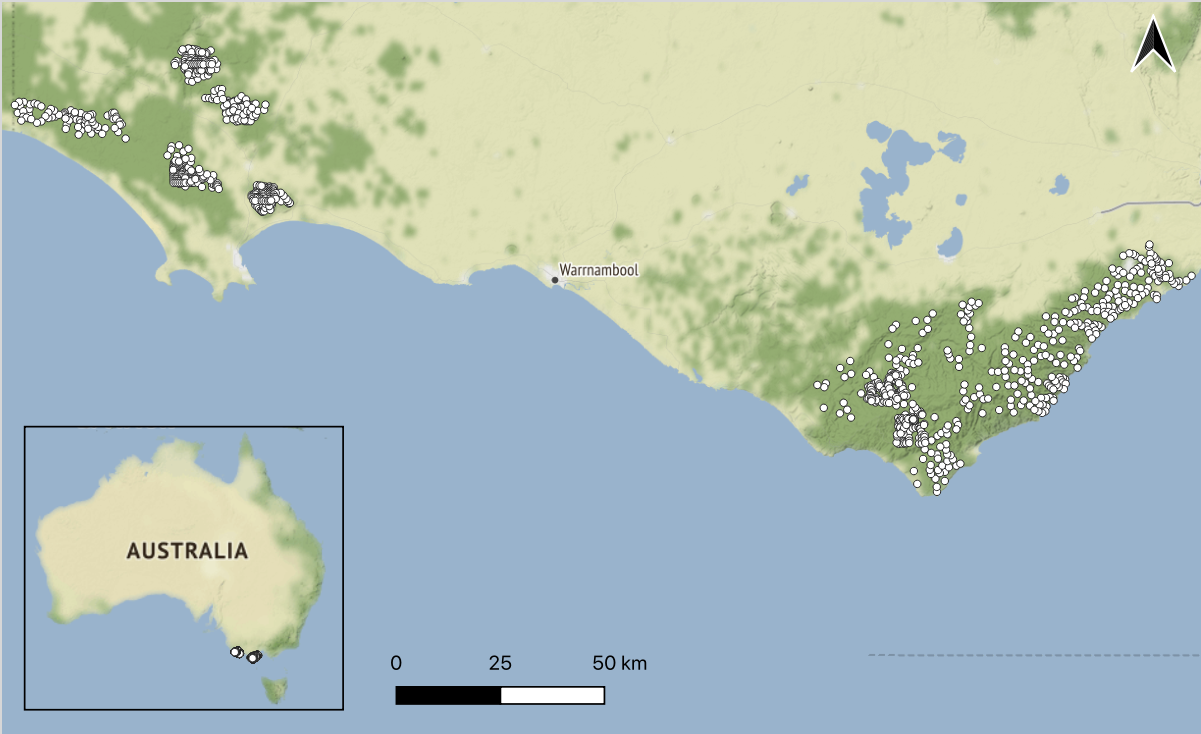
\includegraphics[width=0.8\linewidth]{../figs/map_cams} 

}

\caption{Locations of our study regions in south-west Victoria, Australia. The grids of camera-traps are denoted by white dots. The Glenelg region (38°05'54''S 141°44'41''E) is to the west and Otway Ranges (38°57'82''S 141°68'41''E) to the east. Native vegetation is indicated by dark green, with hill shading. \emph{Map tiles by Stamen Design, under CC BY 3.0, map data by OpenStreetMap, under CC BY SA.}.}\label{fig:diel-map}
\end{figure}

\newpage

\hypertarget{results}{%
\section{RESULTS}\label{results}}

\hypertarget{lethal-suppression-of-foxes}{%
\subsection{Lethal suppression of foxes}\label{lethal-suppression-of-foxes}}

In each model, there was a strong effect of poison fox-baiting on fox spatial activity, particularly in the Glenelg region (Supporting Information Fig. \ref{fig:fox-baits}b). Predicted fox counts on the response scale were reduced by a factor of 12, 24, and 28 in the Glenelg region, as well as a factor of 13, 13, and 8 in the Otway Ranges, for models 1, 2, and 3, respectively. For example, model 2 predicted fox counts in the Glenelg region to range from 0.097 (95\% CI: 0.077 - 0.122) in sites with no fox-baiting, to 0.004 (95\% CI: 0.002 - 0.012) at sites with the maximum poison-bait density; in the Otways ranging from 0.041 (95\% CI: 0.033 - 0.05) - 0.008 (95\% CI: 0.003 - 0.020) across the gradient of poison-bait density.

\hypertarget{how-does-predator-diel-activity-patterns-vary-across-geographic-space-model-1-1}{%
\subsection{How does predator diel activity patterns vary across geographic space? (model 1)}\label{how-does-predator-diel-activity-patterns-vary-across-geographic-space-model-1-1}}

Predator activity varied considerably across space and throughout the 24-hour daily cycle, and there was some variation in the predator diel activity patterns across space. On average, both predators showed similar diel activity patterns, with peaks in activity around sunrise and sunset (i.e., crepuscular), although were more likely to be active during the night than the day (Fig. \ref{fig:diel-st-int}i). On average, the main difference between the species was that fox activity peaked just after sunset and they were less likely to be active during the day than cats. Cats also tended to be more active at sunset relative to sunrise (Fig. \ref{fig:diel-st-int}i).

The interaction between hourly and spatial smooths revealed deviations from marginal diel activity pattern in space, particularly across the two regions, and within the Otway Ranges (Fig. \ref{fig:diel-st-int}). For example, at midday, foxes were less active in the Glenelg region and more active across much of the Otway Ranges (except for the north-east) than the average diel activity pattern. Relative to foxes, cats had slightly more complex (i.e., wiggly) deviations in space from their average diel activity pattern. Most notably, cats were less active during sunset and more active at midnight in the Otway Ranges relative to the Glenelg region (Fig. \ref{fig:diel-st-int}).

\hypertarget{how-does-vegetation-type-and-human-footprint-affect-predator-activity-patterns-model-2-1}{%
\subsection{How does vegetation type and human footprint affect predator activity patterns? (model 2)}\label{how-does-vegetation-type-and-human-footprint-affect-predator-activity-patterns-model-2-1}}

Vegetation type had a strong influence on the spatial and diel activity patterns of foxes and cats, whereas human footprint only affected fox spatial activity. Spatial levels of fox activity were similar across all vegetation types, except wet forests where fox activity was considerably lower. Spatial cat activity was relatively more variable across vegetation types; lowest in heathy woodlands and highest in wet forests (Fig. \ref{fig:diel-veg}b). Diel activity patterns for foxes were similar across all vegetation type except wet forests; in wet forests, foxes were consistently active throughout the daily cycle (Fig. \ref{fig:diel-veg}a). On the other hand, cats were mostly nocturnal (and most active) in wet forests, but largely crepuscular in all other vegetation types (Fig. \ref{fig:diel-veg}a).

There was no evidence that human footprint affected diel activity patterns for either predator species; the interaction term between hour and human footprint index was removed from both models. Fox spatial activity increased linearly with the human footprint index (Supporting Information Fig. \ref{fig:fox-hfi}a), although human footprint did not impact cat spatial activity (the marginal effect of human footprint was also removed from the cat model).

\hypertarget{do-feral-cats-avoid-foxes-in-space-or-time-model-3-1}{%
\subsection{Do feral cats avoid foxes in space or time? (model 3)}\label{do-feral-cats-avoid-foxes-in-space-or-time-model-3-1}}

The model indicated that cats avoided foxes temporally rather than spatially (Fig. \ref{fig:diel-cat-fox}). Fox activity did not impact spatial cat activity in the Otway Ranges, whereas cat spatial activity slightly increased with adjusted fox counts in the Glenelg region.

Across all habitat types, feral cat diel activity patterns changed across gradients of fox activity (Fig. \ref{fig:diel-cat-fox}). In the Glenelg region and Otway dry habitat types, feral cats had a nocturnal-crepuscular diel activity pattern where fox activity was low, but were most active during the day where fox activity was high. In contrast, in the wet forests of the Otway Ranges, feral cats were more strongly nocturnal when fox activity was high, avoiding dawn in particular.

\newpage

\begin{figure}

{\centering 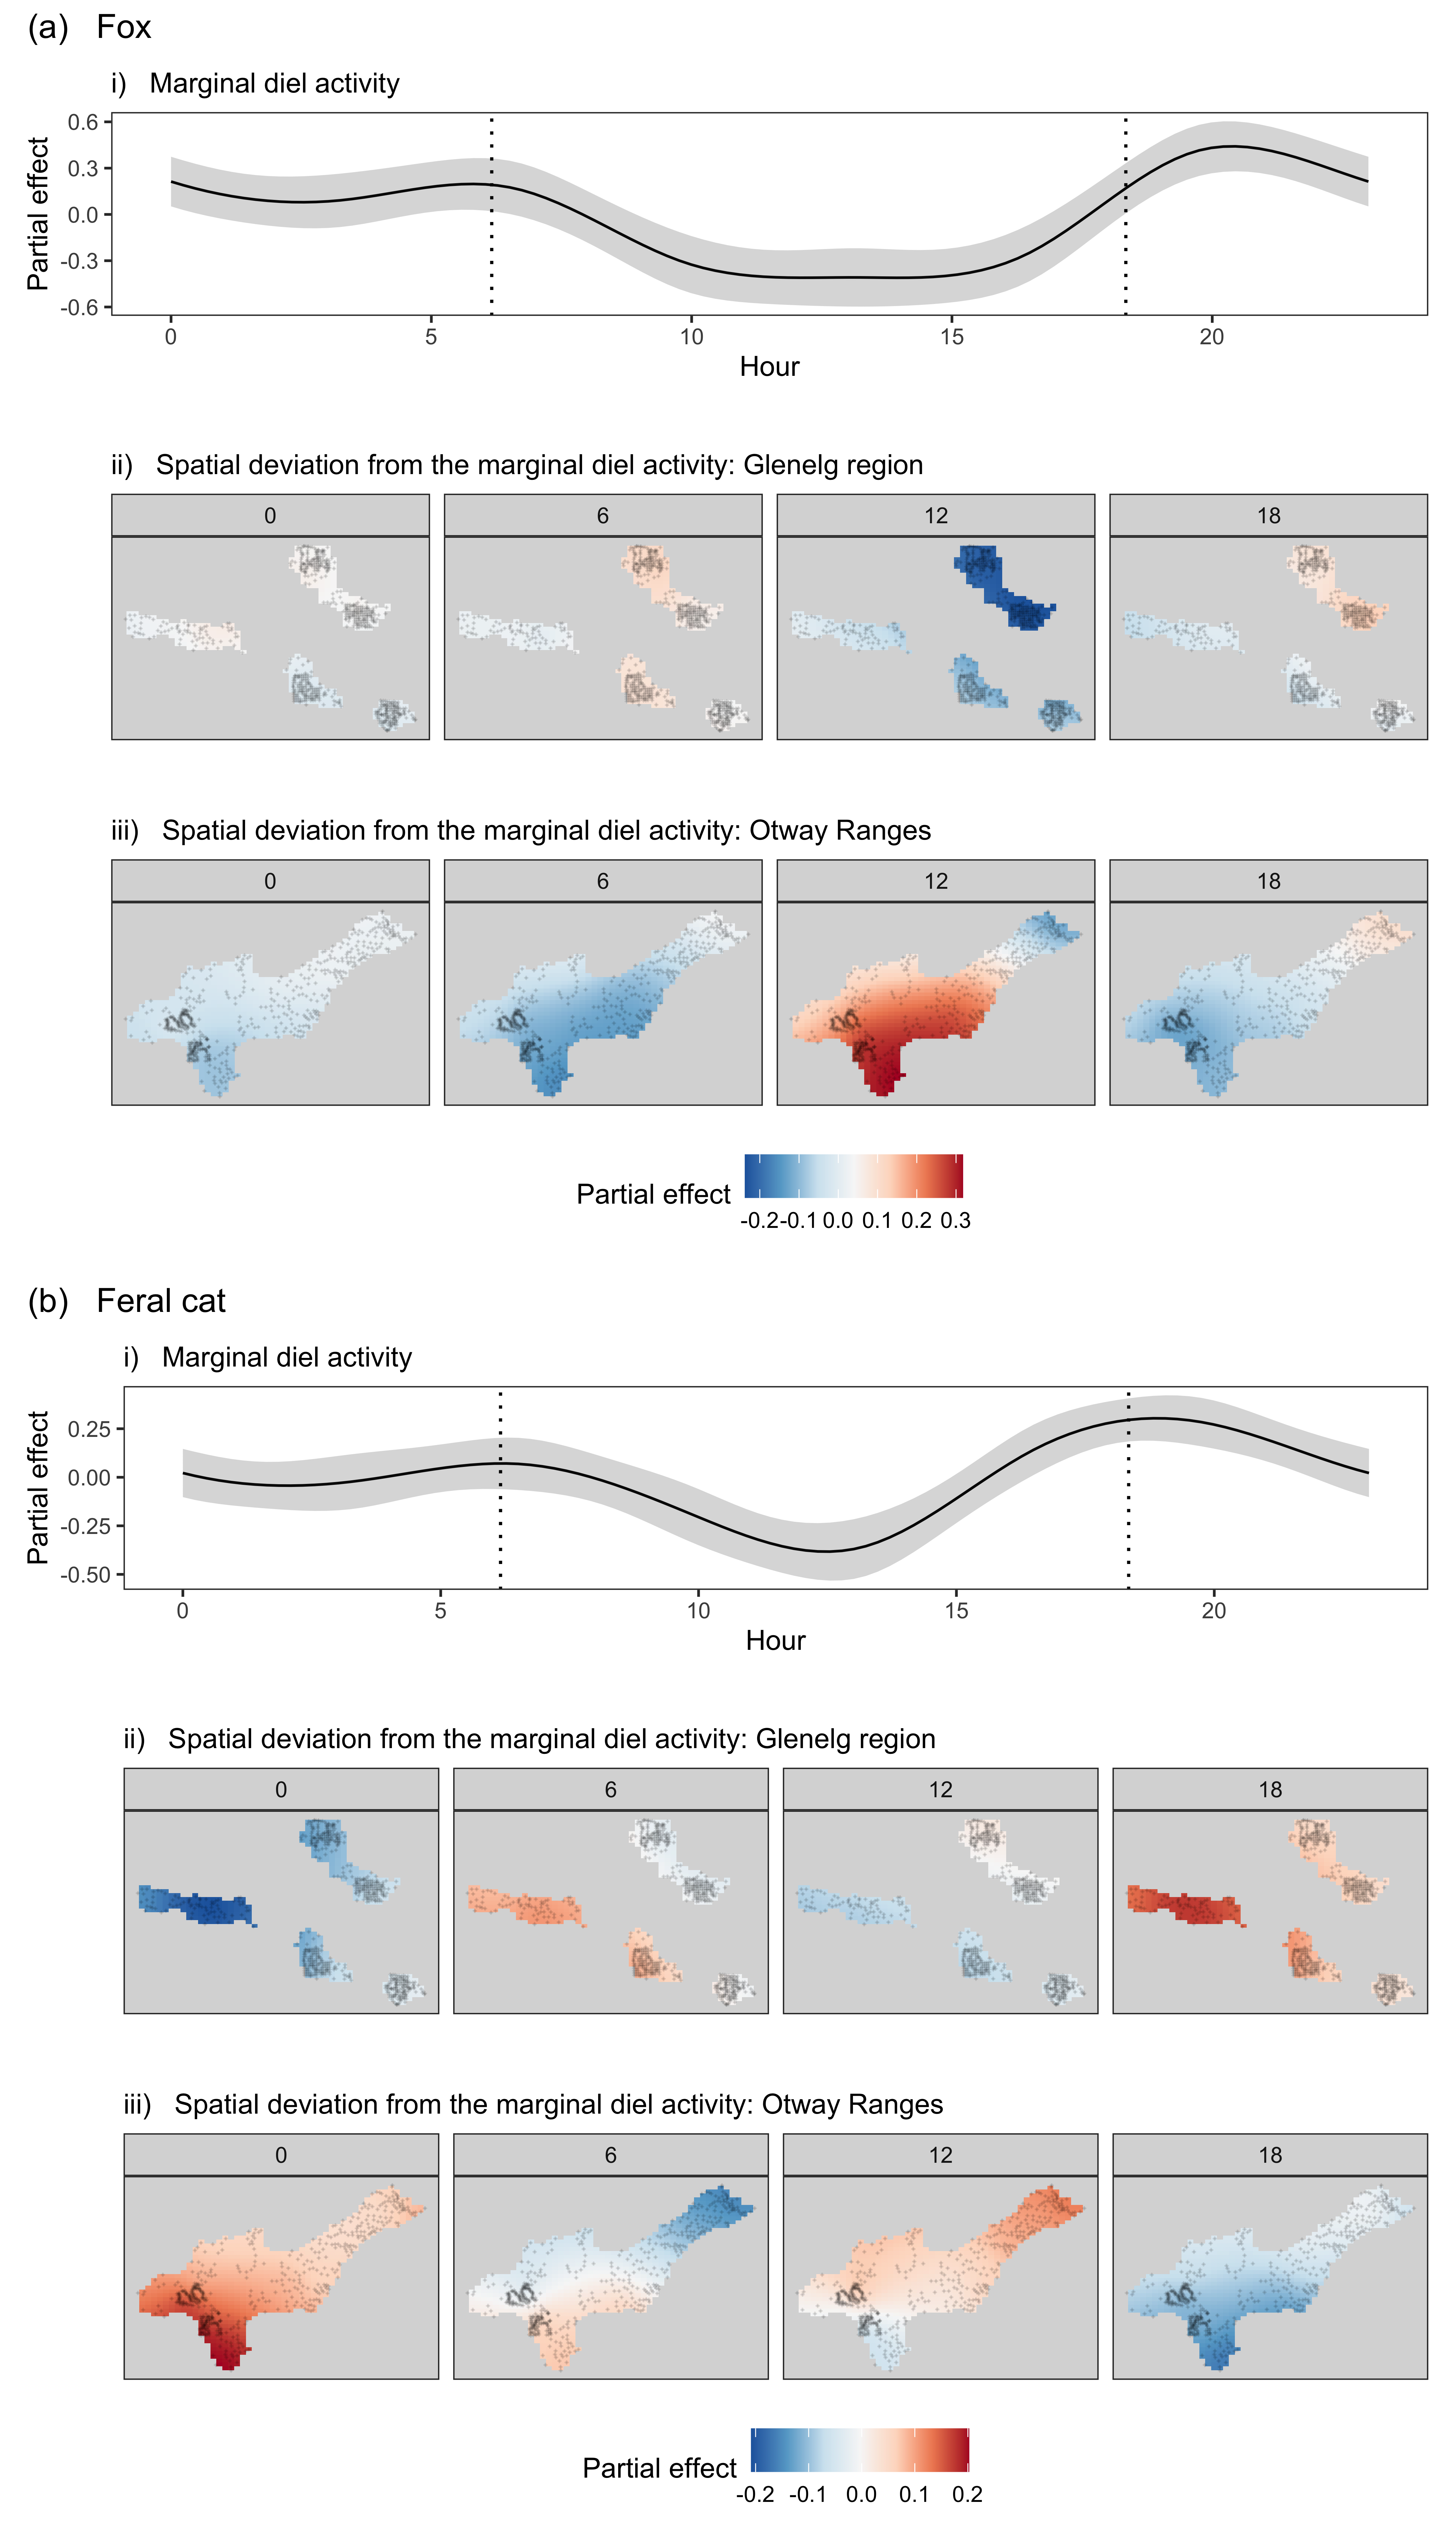
\includegraphics[width=0.7\linewidth]{../figs/spatial_interaction} 

}

\caption{Marginal diel activity (i) and space-time interaction effect in the Glenelg region (ii) and Otway Ranges (iii) at midnight (0), sunrise (6), midday (12) and sunset (18) times for introduced red foxes \textit{Vulpes vulpes} and feral cats \textit{Felis catus}. These effects were estimated by a Generalised Additive Model with a tensor product interaction between spatial and hourly smooths, fit to camera-trap data ('model 1'). Dotted, vertical lines represent average sunrise and sunset times, shaded areas indicate 95\% confidence intervals (i); black dots depict camera-trap sites (ii; iii).}\label{fig:diel-st-int}
\end{figure}

\newpage

\begin{figure}

{\centering 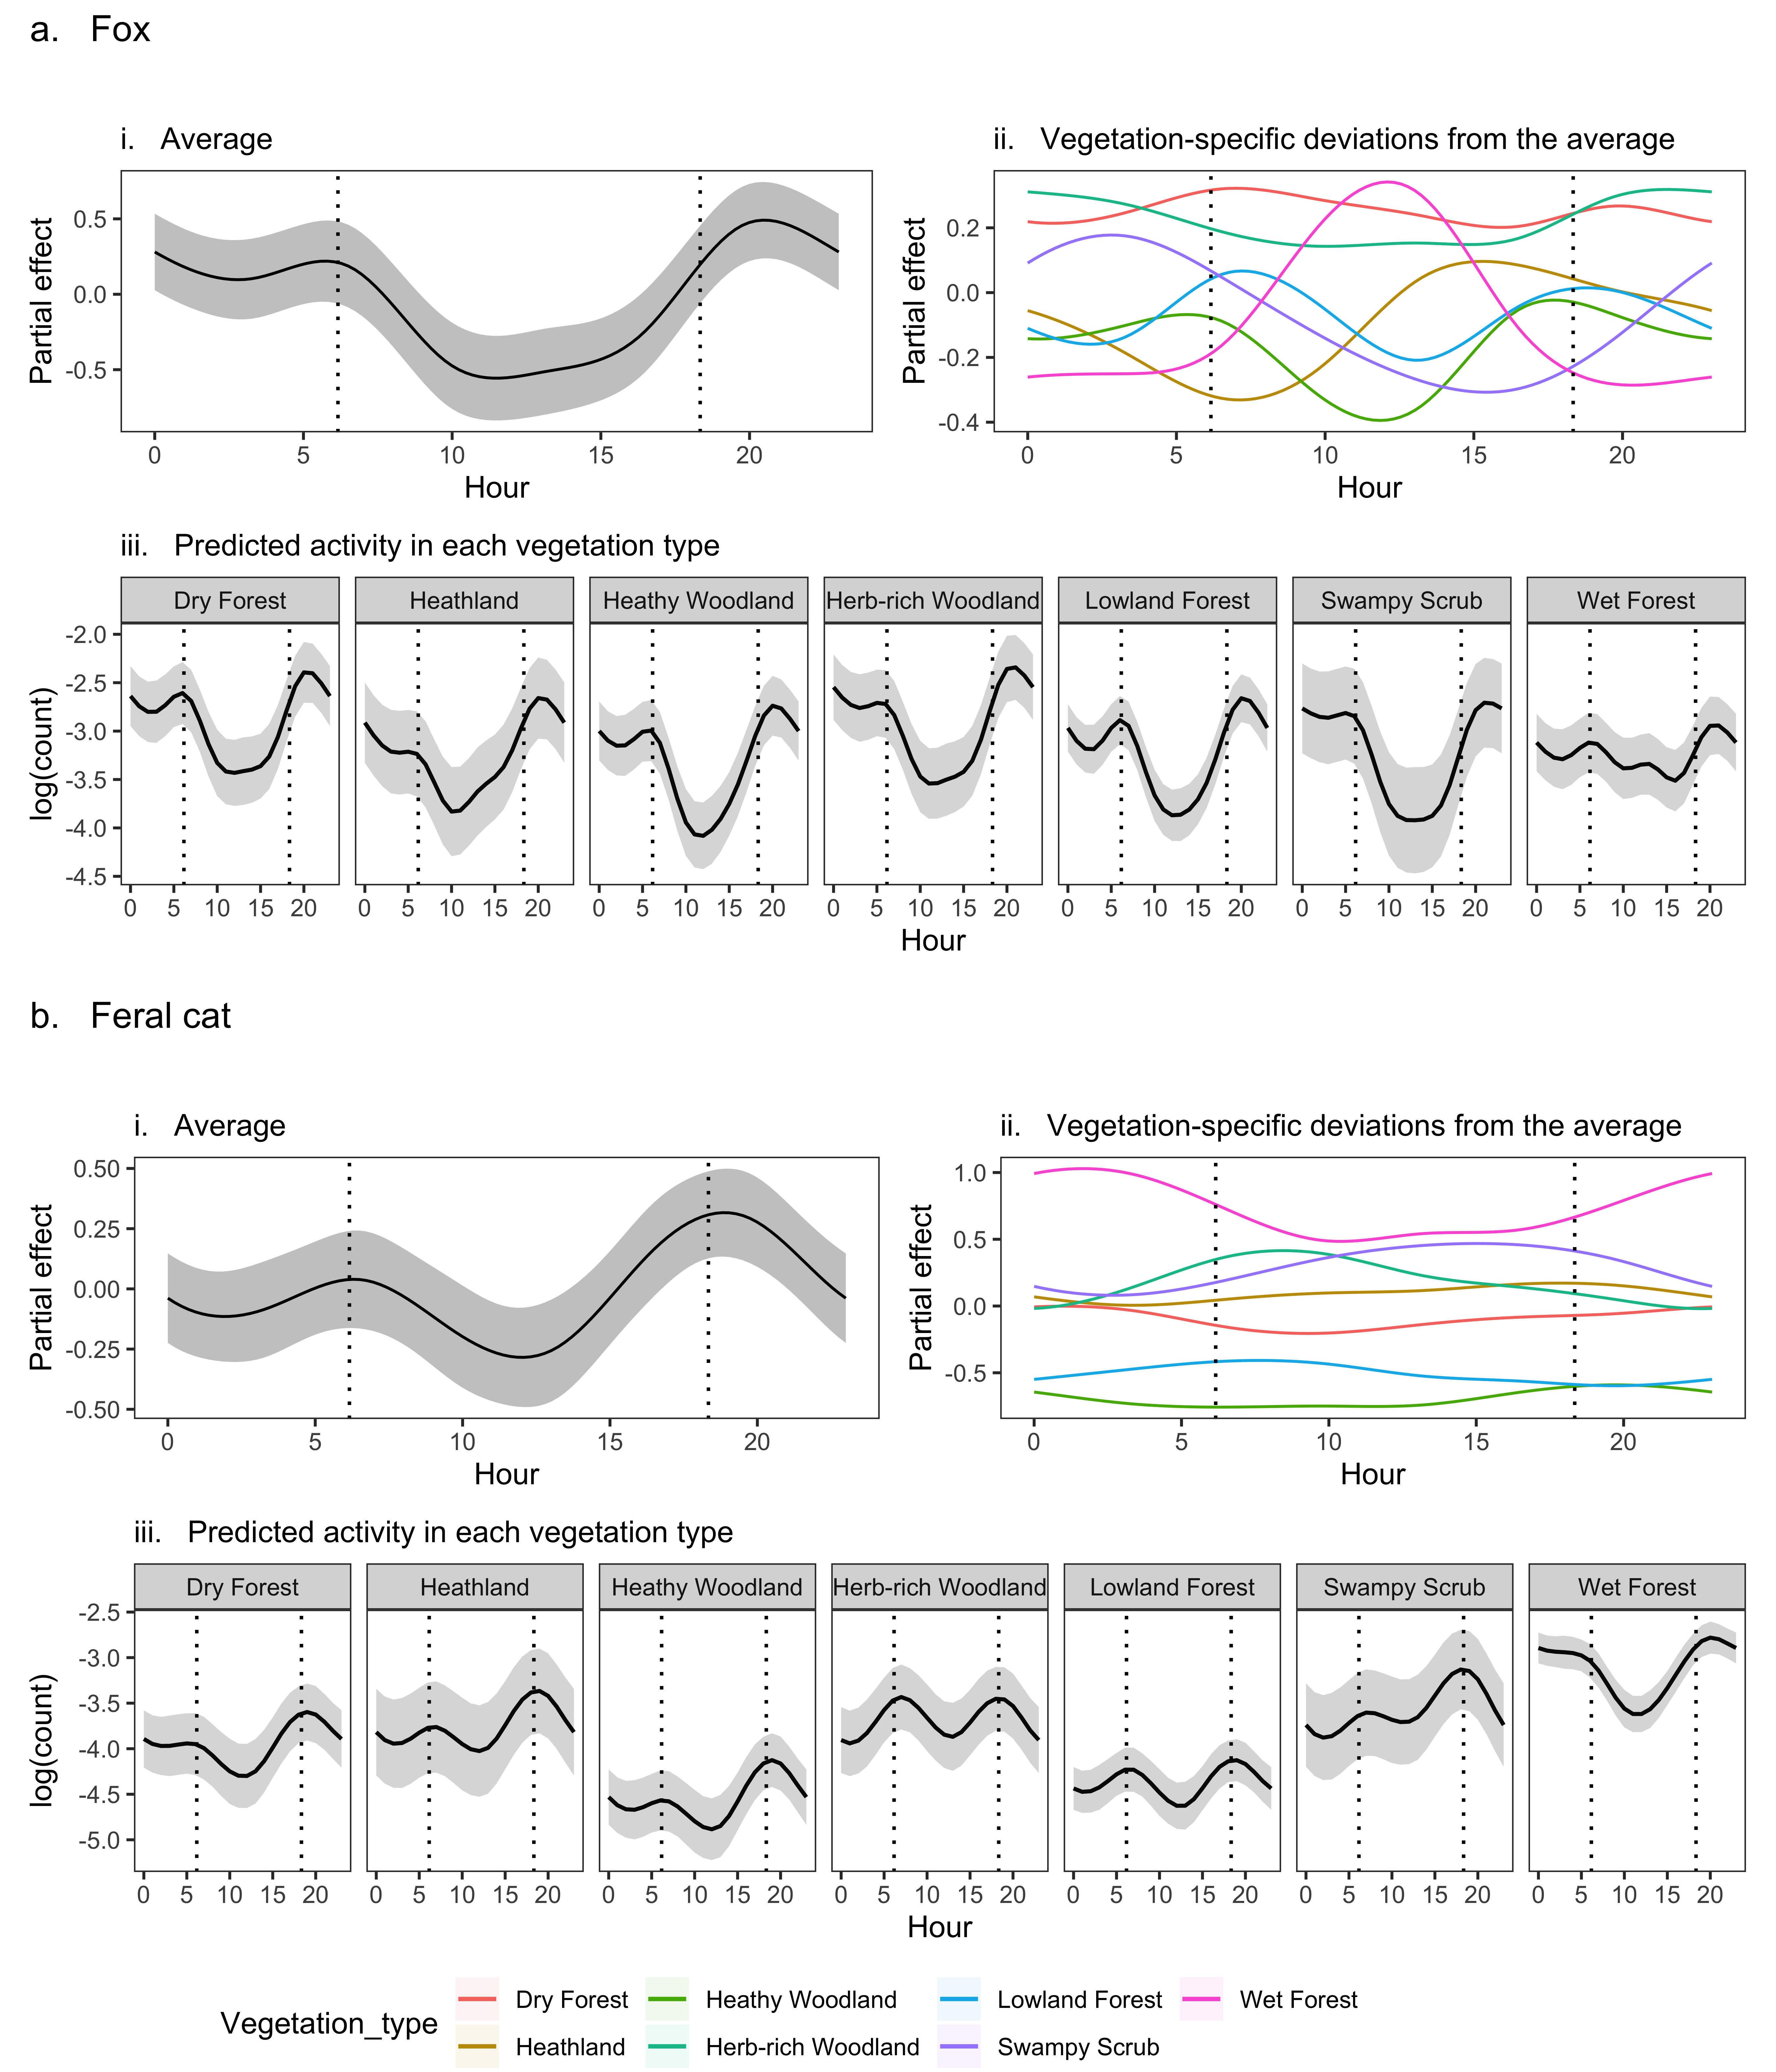
\includegraphics[width=0.8\linewidth]{../figs/predator_veg_leg} 

}

\caption{Red fox \textit{Vulpes vulpes} (a) and feral cat \textit{Felis catus} (b) diel activity patterns overall (i) and across different Ecological Vegetation Class (EVC) groups (ii, iii) in south-west Victoria, Australia. These effects were estimated by a hierarchical Generalised Additive Model with a global smoother for hour (i.e., average response) and group-level smoothers with shared wiggliness for vegetation type (EVC groups), fit to camera-trap data ('model 2'). Dotted, vertical lines represent average sunrise and sunset times. Shaded areas indicate 95\% confidence intervals. Both invasive predators had a crepuscular to nocturnal diel activity pattern on average, with slight deviations across the drier EVC groups and large deviations in wet forests (ii; wet forests shown as pink line). The overall level of activity was relatively consistent across EVC groups for foxes (a – iii), whereas it differed substantially for feral cats (b - iii).}\label{fig:diel-veg}
\end{figure}

\newpage

\begin{figure}

{\centering 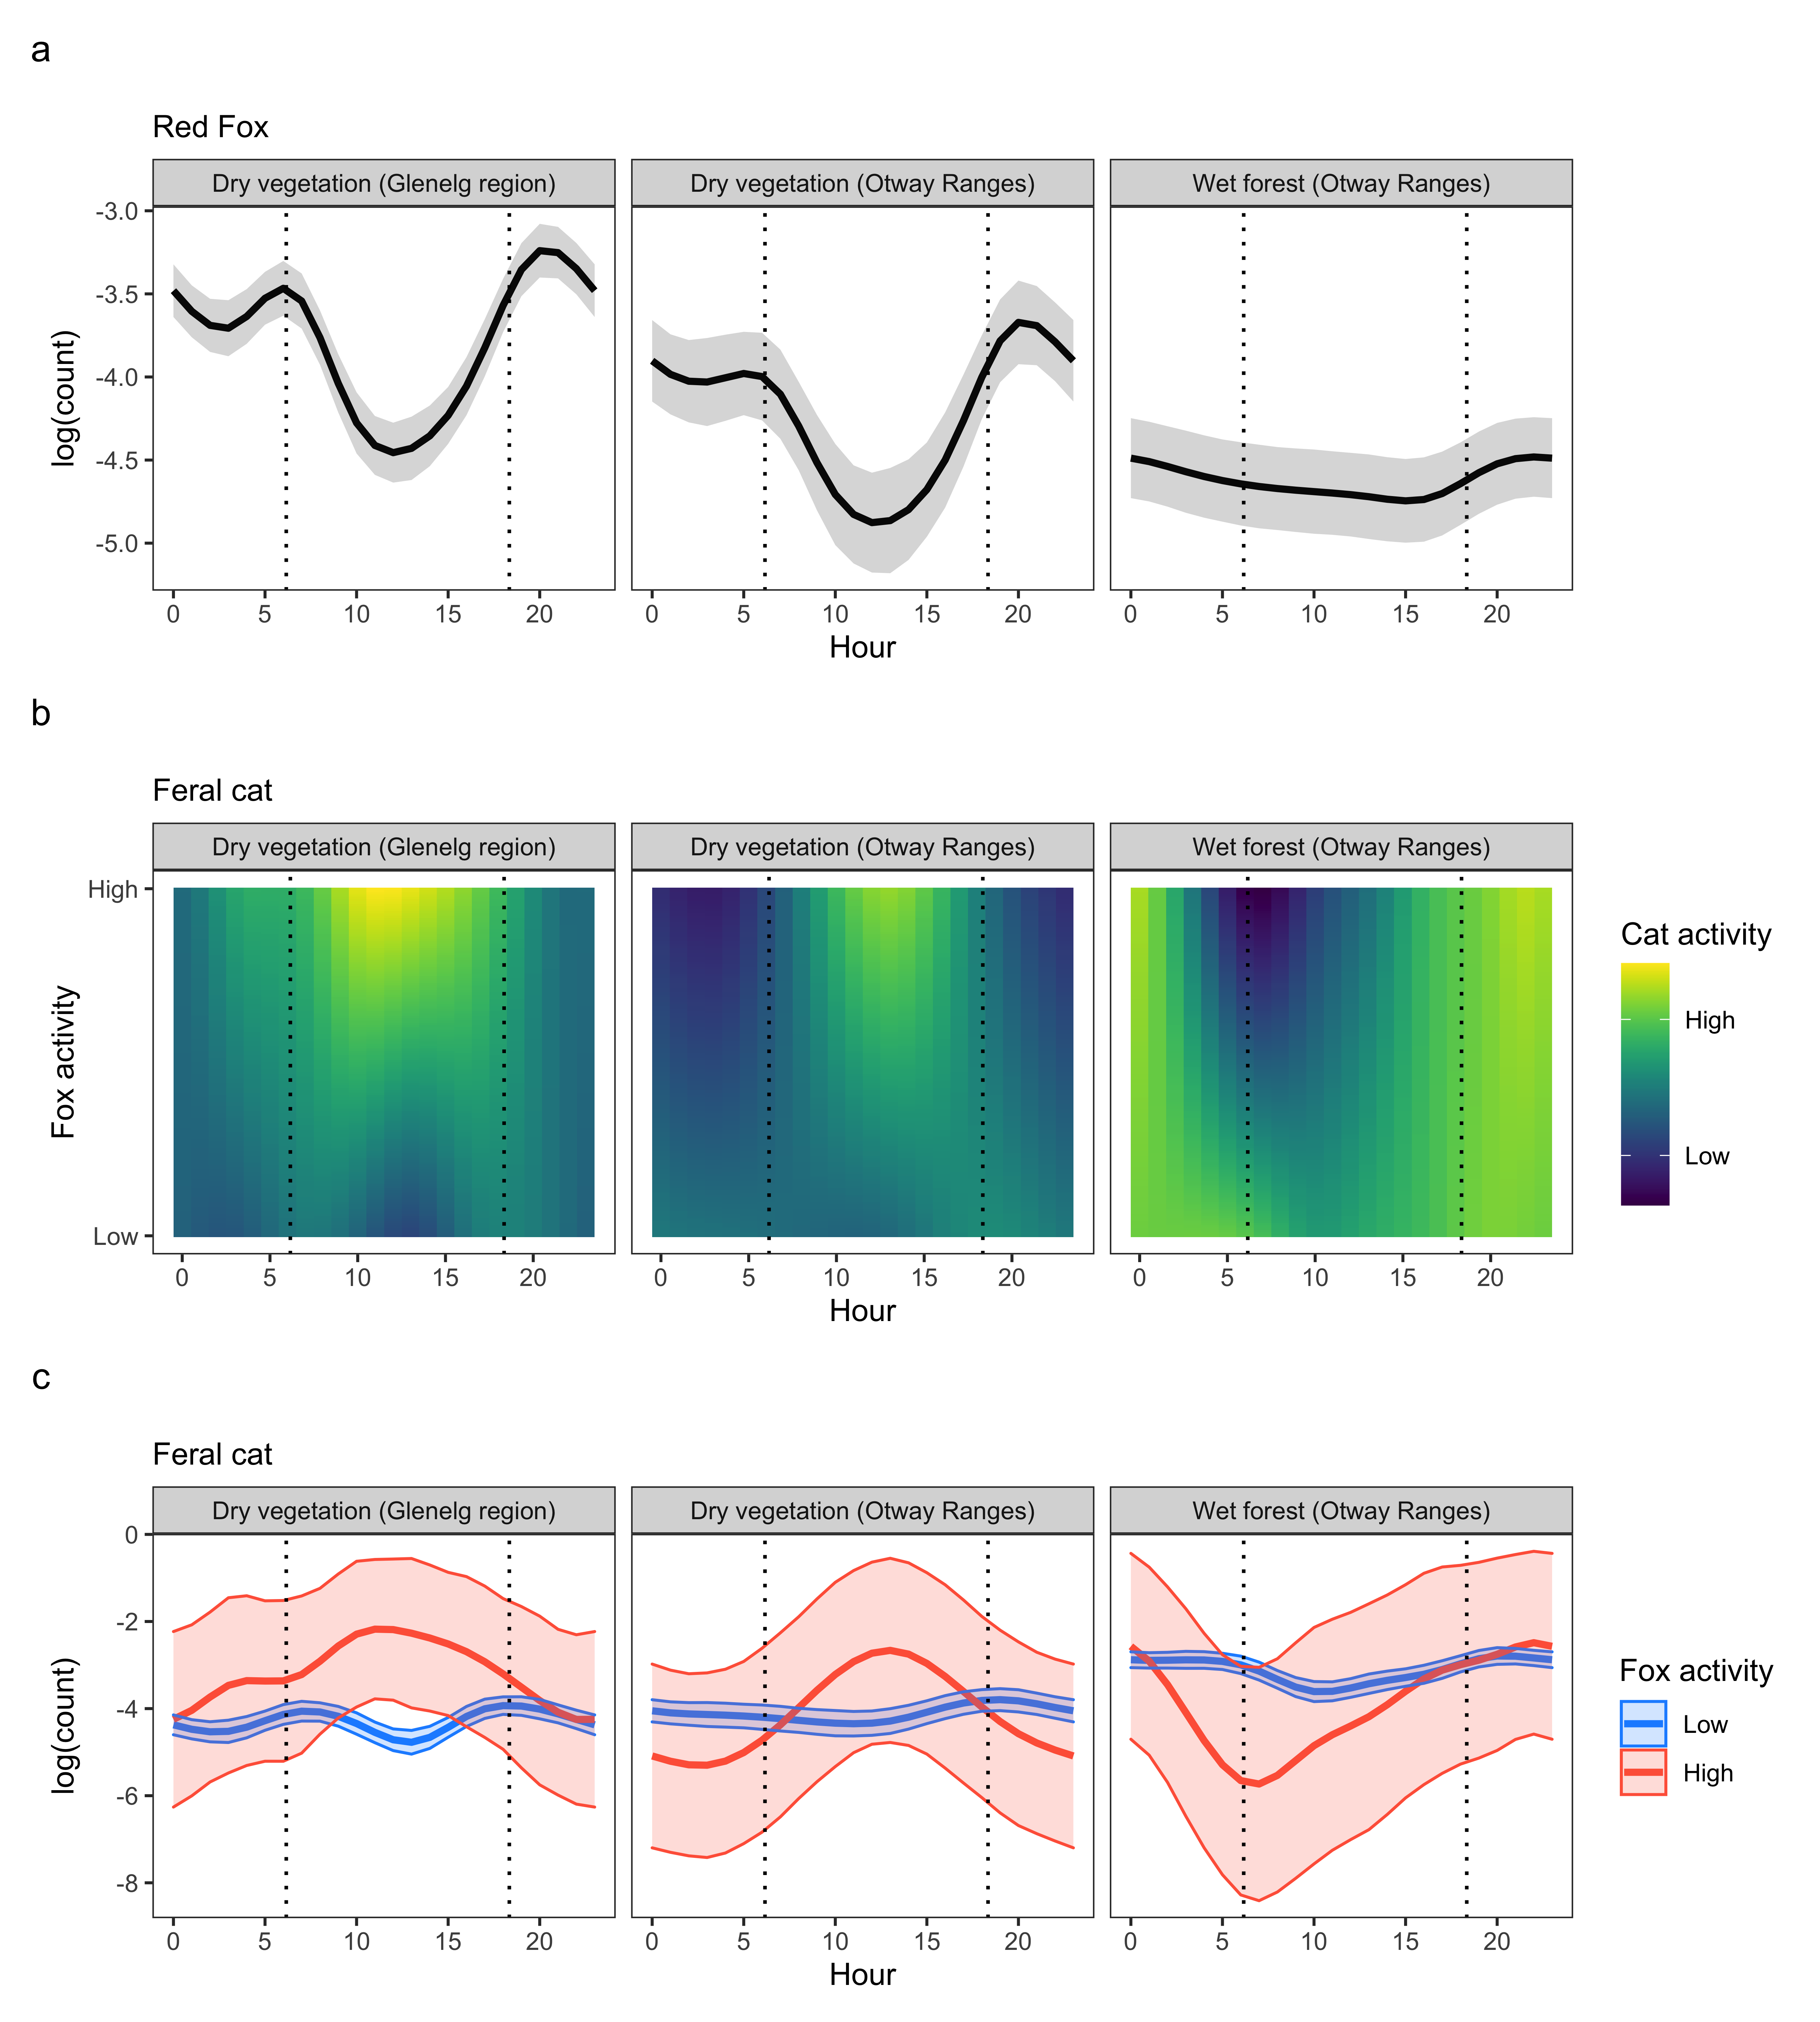
\includegraphics[width=0.8\linewidth]{../figs/cat_fox_count} 

}

\caption{Red fox \textit{Vulpes vulpes} diel activity patterns (a), as well as variation in feral cat \textit{Felis catus} diel activity patterns in response to counts of 'independent' fox detections (log-transformed and survey effort adjusted) across each habitat type in south-west Victoria, Australia (b; c). Effects were estimated by a Generalised Additive Model with a tensor product interaction between hour (cyclical spine) and fox counts adjusted for survey length at each camera-trap ('fox activity'; 'model 3'), fit to camera-trap data. Panels B and C present the same model in two different ways: (b) cat diel activity across the entire continuum of fox activity, (c) cat diel activity patterns at the minimum and maximum fox activity, with associated 95\% confidence intervals (shaded bands). Grey vertical lines represent average sunrise and sunset times. In the Glenelg region, there were more feral cat detections where there were more fox detections, but cat peak diel activity shifted from crepuscular night to pre-dawn and midday (a). In the Otway Ranges, feral cat activity also peaked during the day where fox activity was high in dry vegetation types (b), but was more nocturnal where fox activity was high in the rainforests and wet forests (c).}\label{fig:diel-cat-fox}
\end{figure}

\newpage

\hypertarget{discussion}{%
\section{DISCUSSION}\label{discussion}}

A key question in ecological theory is whether animals are evolutionarily hardwired to occupy particular temporal niches, or have circadian rhythms that are responsive to changing environmental conditions and interactions with other species (Schoener 1974, Daan 1981, Lima and Dill 1990). Here we demonstrate that diel activity patterns are not fixed, but vary across space based on landscape context and fear. In our study, sympatric invasive predators had similar diel activity patterns when averaged across broad regions (i.e., high circular overlap, as did Roshier and Carter 2021), but behaviours varied considerably within landscapes. Foxes were nocturnal in dry habitat types, but showed little variation in activity through the daily cycle in wet forests (Fig. \ref{fig:diel-veg}a). In contrast, cats were mostly nocturnal in wet forests but crepuscular in dry vegetation types (Fig. \ref{fig:diel-veg}b). Within broad habitat types, cats altered their diel activity patterns at sites with higher fox activity towards less-risky times of day (i.e., times when fox activity was lower), however we found no signs of foxes suppressing cat spatial activity (Fig. \ref{fig:diel-cat-fox}). Control programs that reduce invasive fox activity may therefore shift cat diel activity patterns, which in turn may alter cat impacts on native prey species. Quantifying changes in diel activity patterns provides important context for understanding species interactions, which is key for effective ecosystem management (Gaynor et al. 2021).

Shifting diel activity patterns may facilitate spatial coexistence of dominant and subordinate species (Carothers and Jaksić 1984). For cats, altering diel activity patterns to less-preferred times of day may be worthwhile to persist in high-quality habitat. There have been an increasing number of studies which document slight changes in diel activity peaks of subordinate species in response to dominant predators, but few studies have demonstrated predator-induced reversals in diel activity (Kronfeld-Schor and Dayan 2003). Notably, ship rats \emph{Rattus norvegicus} were also found to switch from nocturnal to diurnal behaviour in response to fox activity (Fenn and Macdonald 1995) and a similar nocturnal-diurnal shift was observed in American mink \emph{Neovison vison} following the recolonisation of native predators (Harrington et al. 2009). Our study is particularly unique in that we replicated this behaviour across two separate regions with experimental manipulation, although there was considerable uncertainty in cat diel activity patterns where fox activity was highest (because there were fewer sites with high fox activity relative to low).

For cats in our study, a switch to diurnal behaviour where fox activity was high in the dry vegetation types may have been facilitated by the higher abundance of reptiles in these habitat types relative to wet forests (which are mostly diurnal, Woinarski et al. 2018). At wet forest sites with high fox activity, cats concentrated their activity away from sunrise and sunset towards midnight, despite a diurnal shift appearing to similarly reduce the risk of a fox encounter. In this situation, we expect becoming more nocturnal to be favourable over a diurnal shift because this is when small mammals are active and cats would be least visible to foxes (cats here mostly had black or grey coats, Rees et al. 2023a). Spatial fox activity was twice as low in the wet forests relative to dry habitat types, and so cats were likely under less pressure to radically alter their diel activity patterns. Understanding how these potential avoidance behaviours impacts native prey is a key research priority to improve invasive predator management.

Cats appeared to avoid foxes in time, but we saw no evidence of spatial avoidance (i.e.~no fine-scale negative association between fox and cat spatial activity. In fact, there was some evidence that cat and fox spatial activity was positively correlated in the Glenelg region, suggesting temporal partitioning may facilitate predator co-abundance in quality habitat. Nonetheless, cats may have still avoided foxes spatially, but transiently on the scale of hours to days, or at finer spatial scales than most camera-trap studies can detect (and which telemetry studies can highlight, e.g., Kohl et al. 2019, Smith et al. 2019). Short-term spatial avoidance is quite plausible given foxes mark territories using scats and odours, which cats could tangibly associate with high risk shortly after. Subordinate predators may prefer temporal avoidance of dominant predators (changing diel patterns or transient site avoidance) over longer-term site avoidance when both species have similar resource requirements and share many prey species.

Many species increase nightly activity to avoid humans (Gaynor et al. 2018, Van Scoyoc et al. 2023), however we effect of human footprint on either predator species on our study. This is somewhat unsurprising given there was little variation in human activity among our sites; we studied predators within rugged conservation reserves largely free from human pressures (our camera-trap sites encompassed only the lower 32\% of the total human footprint index range). On the other hand, foxes within our study region often select for human-modified features more during night than day (Hradsky et al. 2017a). Subordinate predators may still prefer to avoid dominant (animal) predators over humans, even when this decision leads to higher mortality rates (Prugh et al. 2023).

A distinction of our study from others is that we modelled potential avoidance behaviours in a simple predator guild, where dominant predator activity was artificially manipulated (suppressed by up to 21-fold). The simple predator guild removes bias from unmodelled impacts of other predators in the system (Levi and Wilmers 2012). Artificial manipulation of the dominant predator also reduces potential bias from differences in niche preferences between the predator species. We also included replication across different habitat types. However, because our study did not consider associations with prey species, we cannot distinguish whether changes in cat diel activity patterns were the result of direct fox avoidance or indirect associations with shared prey. For example, low fox activity may promote the availability of a preferred shared prey species with a diel pattern which differs from those of cats on average, and as a result, cats might shift diel activity patterns at sites with low fox activity to more closely match those of the more abundant prey species. We would expect introduced European rabbits \emph{Oryctolagus cuniculus} and hares \emph{Lepus europaeus} (which are diurnal) to be particularly likely to induce such a response in dry vegetation types (McGregor et al. 2020, Stobo-Wilson et al. 2020), however, rabbits and hares are rare within the natural vegetation of the landscapes we surveyed (only ever being detected at 40 of 1,232 sites) and there is little evidence that predation by foxes suppresses rabbit populations (Norbury and Jones 2015, Scroggie et al. 2018).

Flexible antipredator behaviours make evolutionary sense, but have been rarely demonstrated in terms of spatiotemporal predator avoidance, because this often requires manipulative experiments or at least more complicated models (although, see Relyea 2003, Brown et al. 2013, Cunningham et al. 2019). Our study demonstrates that GAMs offer a powerful tool for modelling continuous shifts in animal activity across both space and time, capable of capturing complex interactions and sharing information across categorical variables. We are only aware of one study which allowed animal diel activity to interact with predation risk as a continuous variable in a GAM (although without allowing for nonlinear shifts via a tensor product or jointly considering spatial activity, Cunningham et al. 2019). Further, complexity penalties are particularly beneficial in assessing spatiotemporal responses, because they are less prone to spurious estimates from small sample sizes or noisy data, and allow multiple hypotheses to be tested within one model without the need for ad-hoc significance testing (e.g., running a separate model for each scenario and comparing with Information Criteria). For example, our model specification allowed cats to respond to fox activity with (a) nonlinear shifts in both spatial and diel activity (as was observed in the Glenelg region), (b) nonlinear shifts in spatial but not diel activity, (c) nonlinear shifts in diel but not spatial activity (as was observed in both habitat types of the Otway Ranges), as well as their respective linear counterparts and also different linear-nonlinear combinations of the first scenario (`model 3'). \textbf{ADD CLOSER}

The alternative approach of simply comparing average diel activity overlap between two species (Ridout and Linkie 2009) would have been misleading for two reasons. Firstly, predator diel activity patterns varied `naturally' across heterogeneous landscapes (requiring avoidance to be tested in wet forests and dry vegetation types separately, Fig. \ref{fig:diel-veg}). Secondly, dominant predator temporal avoidance strategies were not consistently employed, but depended on spatial dominant predator activity and habitat type (Fig. \ref{fig:diel-cat-fox}). Despite their underlying statistical complexity, GAMs in the `mgcv' R-package are straightforward to fit. Our GAM framework for modelling spatiotemporal activity can be used on any species with time-stamped detections, including datasets with categorical or continuous covariates and hierarchical groupings. However, like many other spatiotemporal approaches such as time-to-encounter models, a key limitation is that our GAM approach did not separate the observation processes from the state process. Integrating GAM-like functions into recently developed multispecies spatiotemporal models (e.g., Kellner et al. 2022) would be highly advantageous.

Animal diel activity patterns can be complex, varying across space, habitat types and threat-levels (McCann et al. 2017). Despite telling an important story about how animals interact with each other and the environment, detection times are commonly discarded from statistical analyses of camera-trap data. When considered, diel activity patterns are predominantly estimated at the population-level, overlooking finer-scale behaviours that can affect fitness, survival and ecosystem-impacts. Our results demonstrate the importance of (a) considering diel activity in regards to species interactions, (b) modelling changes in animal behaviour rather than overlap with other species, and (c) testing avoidance behaviours within a joint spatiotemporal framework. Our study adds to the growing body of evidence that dominant predators may cause fear which is powerful enough to reverse the diel activity patterns of subordinate species (Kronfeld-Schor and Dayan 2003), and crucially, demonstrates that these effects are habitat-dependent.

\newpage

\hypertarget{references}{%
\section*{REFERENCES}\label{references}}
\addcontentsline{toc}{section}{REFERENCES}

\hypertarget{refs}{}
\begin{CSLReferences}{1}{0}
\leavevmode\vadjust pre{\hypertarget{ref-azzou2021sparse}{}}%
Ait Kaci Azzou, S. et al. 2021. \href{https://doi.org/10.1111/ecog.05411}{A sparse observation model to quantify species distributions and their overlap in space and time}. - Ecography 44: 928--940.

\leavevmode\vadjust pre{\hypertarget{ref-algar2004feral}{}}%
Algar, D. and Burrows, N. 2004. Feral cat control research: Western shield review--february 2003. - Conservation Science Western Australia in press.

\leavevmode\vadjust pre{\hypertarget{ref-allen2022fear}{}}%
Allen, M. C. et al. 2022. \href{https://doi.org/10.1073/pnas.2112404119}{Fear of predators in free-living wildlife reduces population growth over generations}. - Proceedings of the National Academy of Sciences 119: e2112404119.

\leavevmode\vadjust pre{\hypertarget{ref-basille2015plastic}{}}%
Basille, M. et al. 2015. \href{https://doi.org/10.1890/14-1706.1}{Plastic response of fearful prey to the spatiotemporal dynamics of predator distribution}. - Ecology 96: 2622--2631.

\leavevmode\vadjust pre{\hypertarget{ref-maptools}{}}%
Bivand, R. and Lewin-Koh, N. 2021. \href{https://CRAN.R-project.org/package=maptools}{Maptools: Tools for handling spatial objects}.

\leavevmode\vadjust pre{\hypertarget{ref-brown1999ecology}{}}%
Brown, J. S. et al. 1999. \href{https://doi.org/10.2307/1383287}{The ecology of fear: Optimal foraging, game theory, and trophic interactions}. - Journal of Mammalogy 80: 385--399.

\leavevmode\vadjust pre{\hypertarget{ref-brown2013phenotypically}{}}%
Brown, G. E. et al. 2013. \href{https://doi.org/10.1098/rspb.2012.2712}{Phenotypically plastic neophobia: A response to variable predation risk}. - Proceedings of the Royal Society B: Biological Sciences 280: 20122712.

\leavevmode\vadjust pre{\hypertarget{ref-carothers1984time}{}}%
Carothers, J. H. and Jaksić, F. M. 1984. \href{https://doi.org/10.2307/3544413}{Time as a niche difference: The role of interference competition}. - Oikos: 403--406.

\leavevmode\vadjust pre{\hypertarget{ref-creel2008relationships}{}}%
Creel, S. and Christianson, D. 2008. \href{https://doi.org/10.1016/j.tree.2007.12.004}{Relationships between direct predation and risk effects}. - Trends in Ecology \& Evolution 23: 194--201.

\leavevmode\vadjust pre{\hypertarget{ref-cunningham2019temporal}{}}%
Cunningham, C. X. et al. 2019. \href{https://doi.org/10.1111/ecog.04485}{Temporal partitioning of activity: Rising and falling top-predator abundance triggers community-wide shifts in diel activity}. - Ecography 42: 2157--2168.

\leavevmode\vadjust pre{\hypertarget{ref-daan1981adaptive}{}}%
Daan, S. 1981. \href{https://doi.org/10.1007/978-1-4615-6552-9_15}{Adaptive daily strategies in behavior}. - In: Biological rhythms. Springer Publishing, pp. 275--298.

\leavevmode\vadjust pre{\hypertarget{ref-davies2021spatial}{}}%
Davies, A. B. et al. 2021. \href{https://doi.org/10.1002/ecy.3319}{Spatial heterogeneity facilitates carnivore coexistence}. - Ecology 102: e03319.

\leavevmode\vadjust pre{\hypertarget{ref-delwp2020bioregions}{}}%
Department of Environment, Land, Water \& Planning 2020. \href{https://www.environment.vic.gov.au/biodiversity/bioregions-and-evc-benchmarks}{{Bioregions and EVC Benchmarks}}.

\leavevmode\vadjust pre{\hypertarget{ref-doherty2017stop}{}}%
Doherty, T. S. and Ritchie, E. G. 2017. \href{https://doi.org/10.1111/conl.12251}{Stop jumping the gun: A call for evidence-based invasive predator management}. - Conservation Letters 10: 15--22.

\leavevmode\vadjust pre{\hypertarget{ref-doherty2016invasive}{}}%
Doherty, T. S. et al. 2016. \href{https://doi.org/10.1073/pnas.1602480113}{Invasive predators and global biodiversity loss}. - Proceedings of the National Academy of Sciences 113: 11261--11265.

\leavevmode\vadjust pre{\hypertarget{ref-estes2011trophic}{}}%
Estes, J. A. et al. 2011. \href{https://doi.org/10.1126/science.1205106}{Trophic downgrading of planet earth}. - Science 333: 301--306.

\leavevmode\vadjust pre{\hypertarget{ref-fancourt2019introduced}{}}%
Fancourt, B. A. et al. 2019. \href{https://doi.org/10.1111/1365-2664.13514}{Do introduced apex predators suppress introduced mesopredators? A multiscale spatiotemporal study of dingoes and feral cats in {A}ustralia suggests not}. - Journal of Applied Ecology 56: 2584--2595.

\leavevmode\vadjust pre{\hypertarget{ref-fenn1995use}{}}%
Fenn, M. G. and Macdonald, D. W. 1995. \href{https://doi.org/10.2307/1382321}{Use of middens by red foxes: Risk reverses rhythms of rats}. - Journal of Mammalogy 76: 130--136.

\leavevmode\vadjust pre{\hypertarget{ref-fleming2022distinctive}{}}%
Fleming, P. A. et al. 2022. \href{https://doi.org/10.1098/rsos.220792}{Distinctive diets of eutherian predators in australia}. - Royal Society Open Science in press.

\leavevmode\vadjust pre{\hypertarget{ref-frey2017investigating}{}}%
Frey, S. et al. 2017. \href{https://doi.org/10.1002/rse2.60}{Investigating animal activity patterns and temporal niche partitioning using camera-trap data: Challenges and opportunities}. - Remote Sensing in Ecology and Conservation 3: 123--132.

\leavevmode\vadjust pre{\hypertarget{ref-gaynor2018influence}{}}%
Gaynor, K. M. et al. 2018. \href{https://doi.org/10.1126/science.aar7121}{The influence of human disturbance on wildlife nocturnality}. - Science 360: 1232--1235.

\leavevmode\vadjust pre{\hypertarget{ref-gaynor2019landscapes}{}}%
Gaynor, K. M. et al. 2019. \href{https://doi.org/10.1016/j.tree.2019.01.004}{Landscapes of fear: Spatial patterns of risk perception and response}. - Trends in Ecology \& Evolution 34: 355--368.

\leavevmode\vadjust pre{\hypertarget{ref-gaynor2021applied}{}}%
Gaynor, K. M. et al. 2021. \href{https://doi.org/10.1111/acv.12629}{An applied ecology of fear framework: Linking theory to conservation practice}. - Animal Conservation 24: 308--321.

\leavevmode\vadjust pre{\hypertarget{ref-glen2005complex}{}}%
Glen, A. S. and Dickman, C. R. 2005. \href{https://doi.org/10.1017/S1464793105006718}{Complex interactions among mammalian carnivores in {{A}ustralia}, and their implications for wildlife management}. - Biological Reviews 80: 387--401.

\leavevmode\vadjust pre{\hypertarget{ref-harmsen2009spatial}{}}%
Harmsen, B. J. et al. 2009. \href{https://doi.org/10.1644/08-MAMM-A-140R.1}{{Spatial and Temporal Interactions of Sympatric Jaguars (Panthera onca) and Pumas (Puma concolor) in a Neotropical Forest}}. - Journal of Mammalogy 90: 612--620.

\leavevmode\vadjust pre{\hypertarget{ref-harrington2009impact}{}}%
Harrington, L. A. et al. 2009. \href{https://doi.org/10.1890/08-0302.1}{The impact of native competitors on an alien invasive: Temporal niche shifts to avoid interspecific aggression}. - Ecology 90: 1207--1216.

\leavevmode\vadjust pre{\hypertarget{ref-DHARMa}{}}%
Hartig, F. 2020. \href{https://CRAN.R-project.org/package=DHARMa}{DHARMa: Residual diagnostics for hierarchical (multi-level / mixed) regression models}.

\leavevmode\vadjust pre{\hypertarget{ref-hradsky2017human}{}}%
Hradsky, B. A. et al. 2017a. \href{https://doi.org/10.1038/s41598-017-12464-7}{Human-modified habitats facilitate forest-dwelling populations of an invasive predator, \emph{{V}ulpes vulpes}}. - Scientific Reports 7: 1--12.

\leavevmode\vadjust pre{\hypertarget{ref-hradsky2017bayesian}{}}%
Hradsky, B. A. et al. 2017b. \href{https://esajournals.onlinelibrary.wiley.com/doi/abs/10.1002/ecs2.1926}{Bayesian networks elucidate interactions between fire and other drivers of terrestrial fauna distributions}. - Ecosphere 8: e01926.

\leavevmode\vadjust pre{\hypertarget{ref-hunter2018not}{}}%
Hunter, D. O. et al. 2018. \href{https://doi.org/10.1111/mam.12115}{Not all predators are equal: A continent-scale analysis of the effects of predator control on {{A}ustralian} mammals}. - Mammal Review 48: 108--122.

\leavevmode\vadjust pre{\hypertarget{ref-iannarilli2019lorelograms}{}}%
Iannarilli, F. et al. 2019. \href{https://doi.org/10.1111/2041-210X.13308}{Using lorelograms to measure and model correlation in binary data: Applications to ecological studies}. - Methods in Ecology and Evolution 10: 2153--2162.

\leavevmode\vadjust pre{\hypertarget{ref-kauffman2007landscape}{}}%
Kauffman, M. J. et al. 2007. \href{https://doi.org/10.1111/j.1461-0248.2007.01059.x}{Landscape heterogeneity shapes predation in a newly restored predator--prey system}. - Ecology Letters 10: 690--700.

\leavevmode\vadjust pre{\hypertarget{ref-kellner2022two}{}}%
Kellner, K. F. et al. 2022. \href{https://doi.org/10.1007/s13253-021-00482-y}{A two-species occupancy model with a continuous-time detection process reveals spatial and temporal interactions}. - Journal of Agricultural, Biological and Environmental Statistics 27: 321--338.

\leavevmode\vadjust pre{\hypertarget{ref-kohl2019prey}{}}%
Kohl, M. T. et al. 2019. \href{https://doi.org/10.1111/ele.13319}{Do prey select for vacant hunting domains to minimize a multi-predator threat?} - Ecology Letters 22: 1724--1733.

\leavevmode\vadjust pre{\hypertarget{ref-kronfeld2003partitioning}{}}%
Kronfeld-Schor, N. and Dayan, T. 2003. \href{https://doi.org/10.1146/annurev.ecolsys.34.011802.132435}{Partitioning of time as an ecological resource}. - Annual Review of Ecology, Evolution, and Systematics 34: 153--181.

\leavevmode\vadjust pre{\hypertarget{ref-levi2012wolves}{}}%
Levi, T. and Wilmers, C. C. 2012. \href{https://doi.org/10.1890/11-0165.1}{Wolves--coyotes--foxes: A cascade among carnivores}. - Ecology 93: 921--929.

\leavevmode\vadjust pre{\hypertarget{ref-lima1990behavioral}{}}%
Lima, S. L. and Dill, L. M. 1990. \href{https://doi.org/10.1139/z90-092}{Behavioral decisions made under the risk of predation: A review and prospectus}. - Canadian Journal of Zoology 68: 619--640.

\leavevmode\vadjust pre{\hypertarget{ref-lima1999temporal}{}}%
Lima, S. L. and Bednekoff, P. A. 1999. \href{https://doi.org/10.1086/303202}{Temporal variation in danger drives antipredator behavior: The predation risk allocation hypothesis}. - The American Naturalist 153: 649--659.

\leavevmode\vadjust pre{\hypertarget{ref-mccann2017temporal}{}}%
McCann, N. P. et al. 2017. \href{https://doi.org/10.1111/ecog.02742}{Temporal scaling in analysis of animal activity}. - Ecography 40: 1436--1444.

\leavevmode\vadjust pre{\hypertarget{ref-mcgregor2020short}{}}%
McGregor, H. et al. 2020. \href{https://doi.org/10.1007/s10530-019-02131-5}{The short-term response of feral cats to rabbit population decline: Are alternative native prey more at risk?} - Biological Invasions 22: 799--811.

\leavevmode\vadjust pre{\hypertarget{ref-miller2014finite}{}}%
Miller, D. L. and Wood, S. N. 2014. \href{https://doi.org/10.1007/s10651-014-0277-4}{Finite area smoothing with generalized distance splines}. - Environmental and Ecological Statistics 21: 715--731.

\leavevmode\vadjust pre{\hypertarget{ref-molsher2017mesopredator}{}}%
Molsher, R. et al. 2017. \href{https://doi.org/10.1371/journal.pone.0168460}{Mesopredator management: Effects of red fox control on the abundance, diet and use of space by feral cats}. - PLoS One 12: e0168460.

\leavevmode\vadjust pre{\hypertarget{ref-moseby2011use}{}}%
Moseby, K. et al. 2011. \href{https://doi.org/10.1071/WR10236}{The use of poison baits to control feral cats and red foxes in arid {South Australia} II. Bait type, placement, lures and non-target uptake}. - Wildlife Research 38: 350--358.

\leavevmode\vadjust pre{\hypertarget{ref-niedballa2019assessing}{}}%
Niedballa, J. et al. 2019. \href{https://doi.org/10.1002/rse2.107}{Assessing analytical methods for detecting spatiotemporal interactions between species from camera trapping data}. - Remote Sensing in Ecology and Conservation 5: 272--285.

\leavevmode\vadjust pre{\hypertarget{ref-norbury2015pests}{}}%
Norbury, G. and Jones, C. 2015. \href{https://doi.org/10.1111/mam.12034}{Pests controlling pests: Does predator control lead to greater {E}uropean rabbit abundance in {A}ustralasia?} - Mammal Review 45: 79--87.

\leavevmode\vadjust pre{\hypertarget{ref-parsons2022effect}{}}%
Parsons, A. W. et al. 2022. \href{https://doi.org/10.1002/ecs2.3993}{The effect of urbanization on spatiotemporal interactions between gray foxes and coyotes}. - Ecosphere 13: e3993.

\leavevmode\vadjust pre{\hypertarget{ref-pedersen2019hierarchical}{}}%
Pedersen, E. J. et al. 2019. \href{https://doi.org/10.7717/peerj.6876}{Hierarchical generalized additive models in ecology: An introduction with mgcv}. - PeerJ 7: e6876.

\leavevmode\vadjust pre{\hypertarget{ref-preisser2005scared}{}}%
Preisser, E. L. et al. 2005. \href{https://doi.org/10.1890/04-0719}{Scared to death? The effects of intimidation and consumption in predator--prey interactions}. - Ecology 86: 501--509.

\leavevmode\vadjust pre{\hypertarget{ref-prugh2009rise}{}}%
Prugh, L. R. et al. 2009. \href{https://doi.org/10.1525/bio.2009.59.9.9}{The rise of the mesopredator}. - Bioscience 59: 779--791.

\leavevmode\vadjust pre{\hypertarget{ref-prugh2023fear}{}}%
Prugh, L. R. et al. 2023. \href{https://doi.org/10.1126/science.adf2472}{Fear of large carnivores amplifies human-caused mortality for mesopredators}. - Science 380: 754--758.

\leavevmode\vadjust pre{\hypertarget{ref-R}{}}%
R Core Team 2020. \href{https://www.R-project.org/}{R: A language and environment for statistical computing}. - R Foundation for Statistical Computing.

\leavevmode\vadjust pre{\hypertarget{ref-reddiex2007control}{}}%
Reddiex, B. et al. 2007. \href{https://doi.org/10.1071/WR05102}{Control of pest mammals for biodiversity protection in {{A}ustralia}. I. Patterns of control and monitoring}. - Wildlife Research 33: 691--709.

\leavevmode\vadjust pre{\hypertarget{ref-rees2023mesopredator}{}}%
Rees, M. W. et al. 2023a. \href{https://doi.org/10.1111/1365-2664.14402}{Mesopredator release among invasive predators: Controlling red foxes can increase feral cat density and alter their behaviour}. - Journal of Applied Ecology 60: 1100--1114.

\leavevmode\vadjust pre{\hypertarget{ref-rees2023data}{}}%
Rees, M. W. et al. 2023b. \href{https://doi.org/10.5061/dryad.69p8cz95w}{Data from: Mesopredator release among invasive predators: Controlling red foxes can increase feral cat density and alter their behaviour}.

\leavevmode\vadjust pre{\hypertarget{ref-relyea2003predators}{}}%
Relyea, R. A. 2003. \href{https://doi.org/10.1890/0012-9658(2003)084\%5B1840:PCAPGT\%5D2.0.CO;2}{Predators come and predators go: The reversibility of predator-induced traits}. - Ecology 84: 1840--1848.

\leavevmode\vadjust pre{\hypertarget{ref-ridout2009estimating}{}}%
Ridout, M. S. and Linkie, M. 2009. \href{https://doi.org/10.1198/jabes.2009.08038}{Estimating overlap of daily activity patterns from camera trap data}. - Journal of Agricultural, Biological, and Environmental Statistics 14: 322--337.

\leavevmode\vadjust pre{\hypertarget{ref-risbey1997control}{}}%
Risbey, D. A. et al. 1997. \href{https://doi.org/10.1071/WR96051}{Control of feral cats for nature conservation. I. Field tests of four baiting methods}. - Wildlife Research 24: 319--326.

\leavevmode\vadjust pre{\hypertarget{ref-robley2014long}{}}%
Robley, A. et al. 2014. \href{https://doi.org/10.1016/j.biocon.2014.10.017}{Long-term and large-scale control of the introduced red fox increases native mammal occupancy in {{A}ustralian} forests}. - Biological Conservation 180: 262--269.

\leavevmode\vadjust pre{\hypertarget{ref-robley2019otway}{}}%
Robley, A. et al. 2019. {The Otway Ark: response of predators and native species 2016--2018.}

\leavevmode\vadjust pre{\hypertarget{ref-robley2020glenelg}{}}%
Robley, A. et al. 2020. {Glenelg Ark 2005--2019: long-term predator and native mammal response to predator control.}

\leavevmode\vadjust pre{\hypertarget{ref-roshier2021space}{}}%
Roshier, D. A. and Carter, A. 2021. \href{https://doi.org/10.1002/ecs2.3628}{Space use and interactions of two introduced mesopredators, european red fox and feral cat, in an arid landscape}. - Ecosphere 12: e03628.

\leavevmode\vadjust pre{\hypertarget{ref-schmitz2004trophic}{}}%
Schmitz, O. J. et al. 2004. \href{https://doi.org/10.1111/j.1461-0248.2003.00560.x}{Trophic cascades: The primacy of trait-mediated indirect interactions}. - Ecology Letters 7: 153--163.

\leavevmode\vadjust pre{\hypertarget{ref-schoener1974compression}{}}%
Schoener, T. W. 1974. \href{https://doi.org/10.1073/pnas.71.10.4169}{The compression hypothesis and temporal resource partitioning}. - Proceedings of the National Academy of Sciences 71: 4169--4172.

\leavevmode\vadjust pre{\hypertarget{ref-scroggie2018invasive}{}}%
Scroggie, M. P. et al. 2018. \href{https://doi.org/10.1111/1365-2664.13253}{Invasive prey controlling invasive predators? European rabbit abundance does not determine red fox population dynamics}. - Journal of Applied Ecology 55: 2621--2631.

\leavevmode\vadjust pre{\hypertarget{ref-gratia}{}}%
Simpson, G. L. 2021. \href{https://gavinsimpson.github.io/gratia/}{{g}ratia: Graceful 'ggplot'-based graphics and other functions for GAMs fitted using 'mgcv'}.

\leavevmode\vadjust pre{\hypertarget{ref-smith2019integrating}{}}%
Smith, J. A. et al. 2019. \href{https://doi.org/10.1007/s00442-019-04381-5}{Integrating temporal refugia into landscapes of fear: Prey exploit predator downtimes to forage in risky places}. - Oecologia 189: 883--890.

\leavevmode\vadjust pre{\hypertarget{ref-soule1988reconstructed}{}}%
Soulé, M. E. et al. 1988. \href{https://doi.org/10.1111/j.1523-1739.1988.tb00337.x}{Reconstructed dynamics of rapid extinctions of chaparral-requiring birds in urban habitat islands}. - Conservation Biology 2: 75--92.

\leavevmode\vadjust pre{\hypertarget{ref-stobo2020management}{}}%
Stobo-Wilson, A. M. et al. 2020. \href{https://doi.org/10.1071/WR19237}{Management of invasive mesopredators in the {Flinders Ranges, South {A}ustralia}: Effectiveness and implications}. - Wildlife Research 47: 720--730.

\leavevmode\vadjust pre{\hypertarget{ref-suraci2016fear}{}}%
Suraci, J. P. et al. 2016. \href{https://doi.org/10.1038/ncomms10698}{Fear of large carnivores causes a trophic cascade}. - Nature communications 7: 1--7.

\leavevmode\vadjust pre{\hypertarget{ref-suraci2022beyond}{}}%
Suraci, J. P. et al. 2022. \href{https://doi.org/10.1111/oik.09004}{Beyond spatial overlap: Harnessing new technologies to resolve the complexities of predator--prey interactions}. - Oikos: e09004.

\leavevmode\vadjust pre{\hypertarget{ref-swan2015predicting}{}}%
Swan, M. et al. 2015. \href{https://doi.org/10.1890/14-1533.1}{Predicting faunal fire responses in heterogeneous landscapes: The role of habitat structure}. - Ecological Applications 25: 2293--2305.

\leavevmode\vadjust pre{\hypertarget{ref-van2023influence}{}}%
Van Scoyoc, A. et al. 2023. \href{https://doi.org/10.1111/1365-2656.13892}{The influence of human activity on predator-prey spatiotemporal overlap}. - The Journal of Animal Ecology 92: 1124---1134.

\leavevmode\vadjust pre{\hypertarget{ref-vazquez2019comparing}{}}%
Vazquez, C. et al. 2019. \href{https://doi.org/10.1111/2041-210X.13290}{Comparing diel activity patterns of wildlife across latitudes and seasons: Time transformations using day length}. - Methods in Ecology and Evolution 10: 2057--2066.

\leavevmode\vadjust pre{\hypertarget{ref-venter2016sixteen}{}}%
Venter, O. et al. 2016. \href{https://doi.org/10.1038/ncomms12558}{Sixteen years of change in the global terrestrial human footprint and implications for biodiversity conservation}. - Nature communications 7: 12558.

\leavevmode\vadjust pre{\hypertarget{ref-venter2018last}{}}%
Venter, O. et al. 2018. \href{https://doi.org/10.7927/H46T0JQ4.}{Last of the wild project, version 3 (LWP-3): 2009 human footprint, 2018 release.}

\leavevmode\vadjust pre{\hypertarget{ref-wayne2017recoveries}{}}%
Wayne, A. F. et al. 2017. \href{https://doi.org/10.1093/jmammal/gyw237}{{Recoveries and cascading declines of native mammals associated with control of an introduced predator}}. - Journal of Mammalogy 98: 489--501.

\leavevmode\vadjust pre{\hypertarget{ref-ggplot2}{}}%
Wickham, H. 2016. \href{https://ggplot2.tidyverse.org}{{g}gplot2: Elegant graphics for data analysis}. - Springer-Verlag New York.

\leavevmode\vadjust pre{\hypertarget{ref-willems2009predator}{}}%
Willems, E. P. and Hill, R. A. 2009. \href{https://doi.org/10.1890/08-0765.1}{Predator-specific landscapes of fear and resource distribution: Effects on spatial range use}. - Ecology 90: 546--555.

\leavevmode\vadjust pre{\hypertarget{ref-wirsing2021context}{}}%
Wirsing, A. J. et al. 2021. \href{https://doi.org/10.1111/ele.13614}{The context dependence of non-consumptive predator effects}. - Ecology Letters 24: 113--129.

\leavevmode\vadjust pre{\hypertarget{ref-woinarski2015ongoing}{}}%
Woinarski, J. C. Z. et al. 2015. \href{https://doi.org/10.1073/pnas.1417301112}{Ongoing unraveling of a continental fauna: Decline and extinction of {{A}ustralian} mammals since {European} settlement}. - Proceedings of the National Academy of Sciences 112: 4531--4540.

\leavevmode\vadjust pre{\hypertarget{ref-woinarski2018reptiles}{}}%
Woinarski, J. C. Z. et al. 2018. \href{https://doi.org/10.1071/WR17160}{How many reptiles are killed by cats in {{A}ustralia}?} - Wildlife Research 45: 247--266.

\leavevmode\vadjust pre{\hypertarget{ref-wood2017generalized}{}}%
Wood, S. N. 2017. Generalized additive models: An introduction with r. - CRC press.

\leavevmode\vadjust pre{\hypertarget{ref-wooster2022predator}{}}%
Wooster, E. I. et al. 2022. \href{https://doi.org/10.1111/oik.09059}{Predator protection dampens the landscape of fear}. - Oikos: e09059.

\end{CSLReferences}

\newpage
\beginsupplement
\setcounter{page}{1}

\hypertarget{supporting-information}{%
\section*{SUPPORTING INFORMATION}\label{supporting-information}}
\addcontentsline{toc}{section}{SUPPORTING INFORMATION}

\newpage

\newpage
\blandscape

\begin{table}

\caption{\label{tab:tab-sum}Summary of experimental camera-trap survey designs around fox control in south-west Victoria, Australia.}
\centering
\resizebox{\linewidth}{!}{
\fontsize{10}{12}\selectfont
\begin{tabular}[t]{llllrrrrrrr}
\toprule
Region & Source & Block & Treatment & Surveys & Year from & Year to & Sites & Min. spacing (m) & Mean spacing (m) & Max spacing (m)\\
\midrule
Glenelg & Glenelg Ark & Annya & non-treatment & 7 & 2013 & 2019 & 40 & 683 & 988 & 1509\\
Glenelg & Glenelg Ark & Hotspur & non-treatment & 7 & 2013 & 2019 & 40 & 335 & 817 & 1319\\
Glenelg & Glenelg Ark & LGNP N & non-treatment & 7 & 2013 & 2019 & 40 & 275 & 687 & 1828\\
Glenelg & Glenelg Ark & Cobboboonee & treatment & 7 & 2013 & 2019 & 40 & 362 & 982 & 2351\\
Glenelg & Glenelg Ark & LGNP S & treatment & 7 & 2013 & 2019 & 40 & 502 & 1120 & 2686\\
\addlinespace
Glenelg & Glenelg Ark & Mt Clay & treatment & 7 & 2013 & 2019 & 40 & 178 & 607 & 1068\\
Glenelg & MWR PhD & Annya & non-treatment & 1 & 2018 & 2018 & 110 & 307 & 469 & 623\\
Glenelg & MWR PhD & Hotspur & non-treatment & 1 & 2018 & 2018 & 99 & 242 & 428 & 594\\
Glenelg & MWR PhD & Cobboboonee & treatment & 1 & 2018 & 2018 & 110 & 274 & 452 & 509\\
Glenelg & MWR PhD & Mt Clay & treatment & 1 & 2018 & 2018 & 106 & 209 & 445 & 671\\
\addlinespace
Otways & MWR PhD & North & non-treatment & 3 & 2017 & 2019 & 104 & 238 & 434 & 714\\
Otways & MWR PhD & South & treatment & 3 & 2017 & 2019 & 91 & 86 & 436 & 717\\
Otways & Otway Ark & FA4 & non-treatment & 3 & 2017 & 2019 & 73 & 634 & 1560 & 4150\\
Otways & Otway Ark & FA1 & treatment & 3 & 2016 & 2018 & 80 & 277 & 996 & 1825\\
Otways & Otway Ark & FA2 & treatment & 3 & 2016 & 2018 & 80 & 638 & 938 & 1865\\
\addlinespace
Otways & Otway Ark & FA3 & treatment & 3 & 2016 & 2018 & 140 & 739 & 1491 & 3514\\
\bottomrule
\end{tabular}}
\end{table}

\thispagestyle{empty}
\elandscape
\newpage

\begingroup\fontsize{10}{12}\selectfont

\begin{longtable}[t]{llrrrr}
\caption{\label{tab:diel-tab1}Summary of the number of camera-trap deployments, unique survey sites and 'independent' counts of invasive predator detections across Ecological Vegetation Class groups within the Glenelg and Otway regions, south-west Victoria, Australia.}\\
\toprule
Vegetation & Region & Sites & Deployments & Fox counts & Cat counts\\
\midrule
Dry Forest & Glenelg & 25 & 69 & 347 & 9\\
 & Otways & 111 & 314 & 341 & 158\\
Heathland & Glenelg & 40 & 119 & 265 & 59\\
 & Otways & 3 & 9 & 8 & 6\\
Heathy Woodland & Glenelg & 154 & 424 & 574 & 96\\
\addlinespace
 & Otways & 82 & 256 & 160 & 66\\
Herb-rich Woodland & Glenelg & 59 & 373 & 863 & 198\\
 & Otways & 2 & 6 & 3 & 2\\
Lowland Forest & Glenelg & 383 & 1046 & 1900 & 290\\
 & Otways & 52 & 163 & 190 & 35\\
\addlinespace
Swampy Scrub & Glenelg & 4 & 10 & 19 & 8\\
 & Otways & 36 & 98 & 64 & 88\\
Wet Forest & Otways & 281 & 780 & 715 & 1187\\
\textbf{Total} & \textbf{} & \textbf{1232} & \textbf{3667} & \textbf{5449} & \textbf{2202}\\
\bottomrule
\end{longtable}
\endgroup{}

\newpage

\begingroup\fontsize{10}{12}\selectfont

\begin{longtable}[t]{llrrr}
\caption{\label{tab:diel-tab-fits}Generalised additive model summaries for invasive predator spatiotemporal activity in south-west Victoria, Australia.}\\
\toprule
Species & Model & EDF & dev.expl & r.sq\\
\midrule
fox & 1\_spatial & 98.0605 & 0.0657 & 0.0137\\
fox & 2\_vegetation\_type & 752.9670 & 0.3496 & 0.1155\\
fox & 3\_habitat\_type & 757.1467 & 0.3486 & 0.1138\\
cat & 1\_spatial & 78.4323 & 0.1110 & 0.0367\\
cat & 2\_vegetation\_type & 566.7735 & 0.2301 & 0.0769\\
\addlinespace
cat & 3\_fox\_by\_habitat\_type & 585.8580 & 0.2317 & 0.0779\\
\bottomrule
\multicolumn{5}{l}{\rule{0pt}{1em}\textit{Note: }}\\
\multicolumn{5}{l}{\rule{0pt}{1em}EDF - estimated degrees of freedom of all model terms.}\\
\multicolumn{5}{l}{\rule{0pt}{1em}dev.expl - proportion of the null deviance explained by the model. }\\
\multicolumn{5}{l}{\rule{0pt}{1em}r.sq -  adjusted r-squared value.}\\
\end{longtable}
\endgroup{}

\newpage

\begin{figure}

{\centering 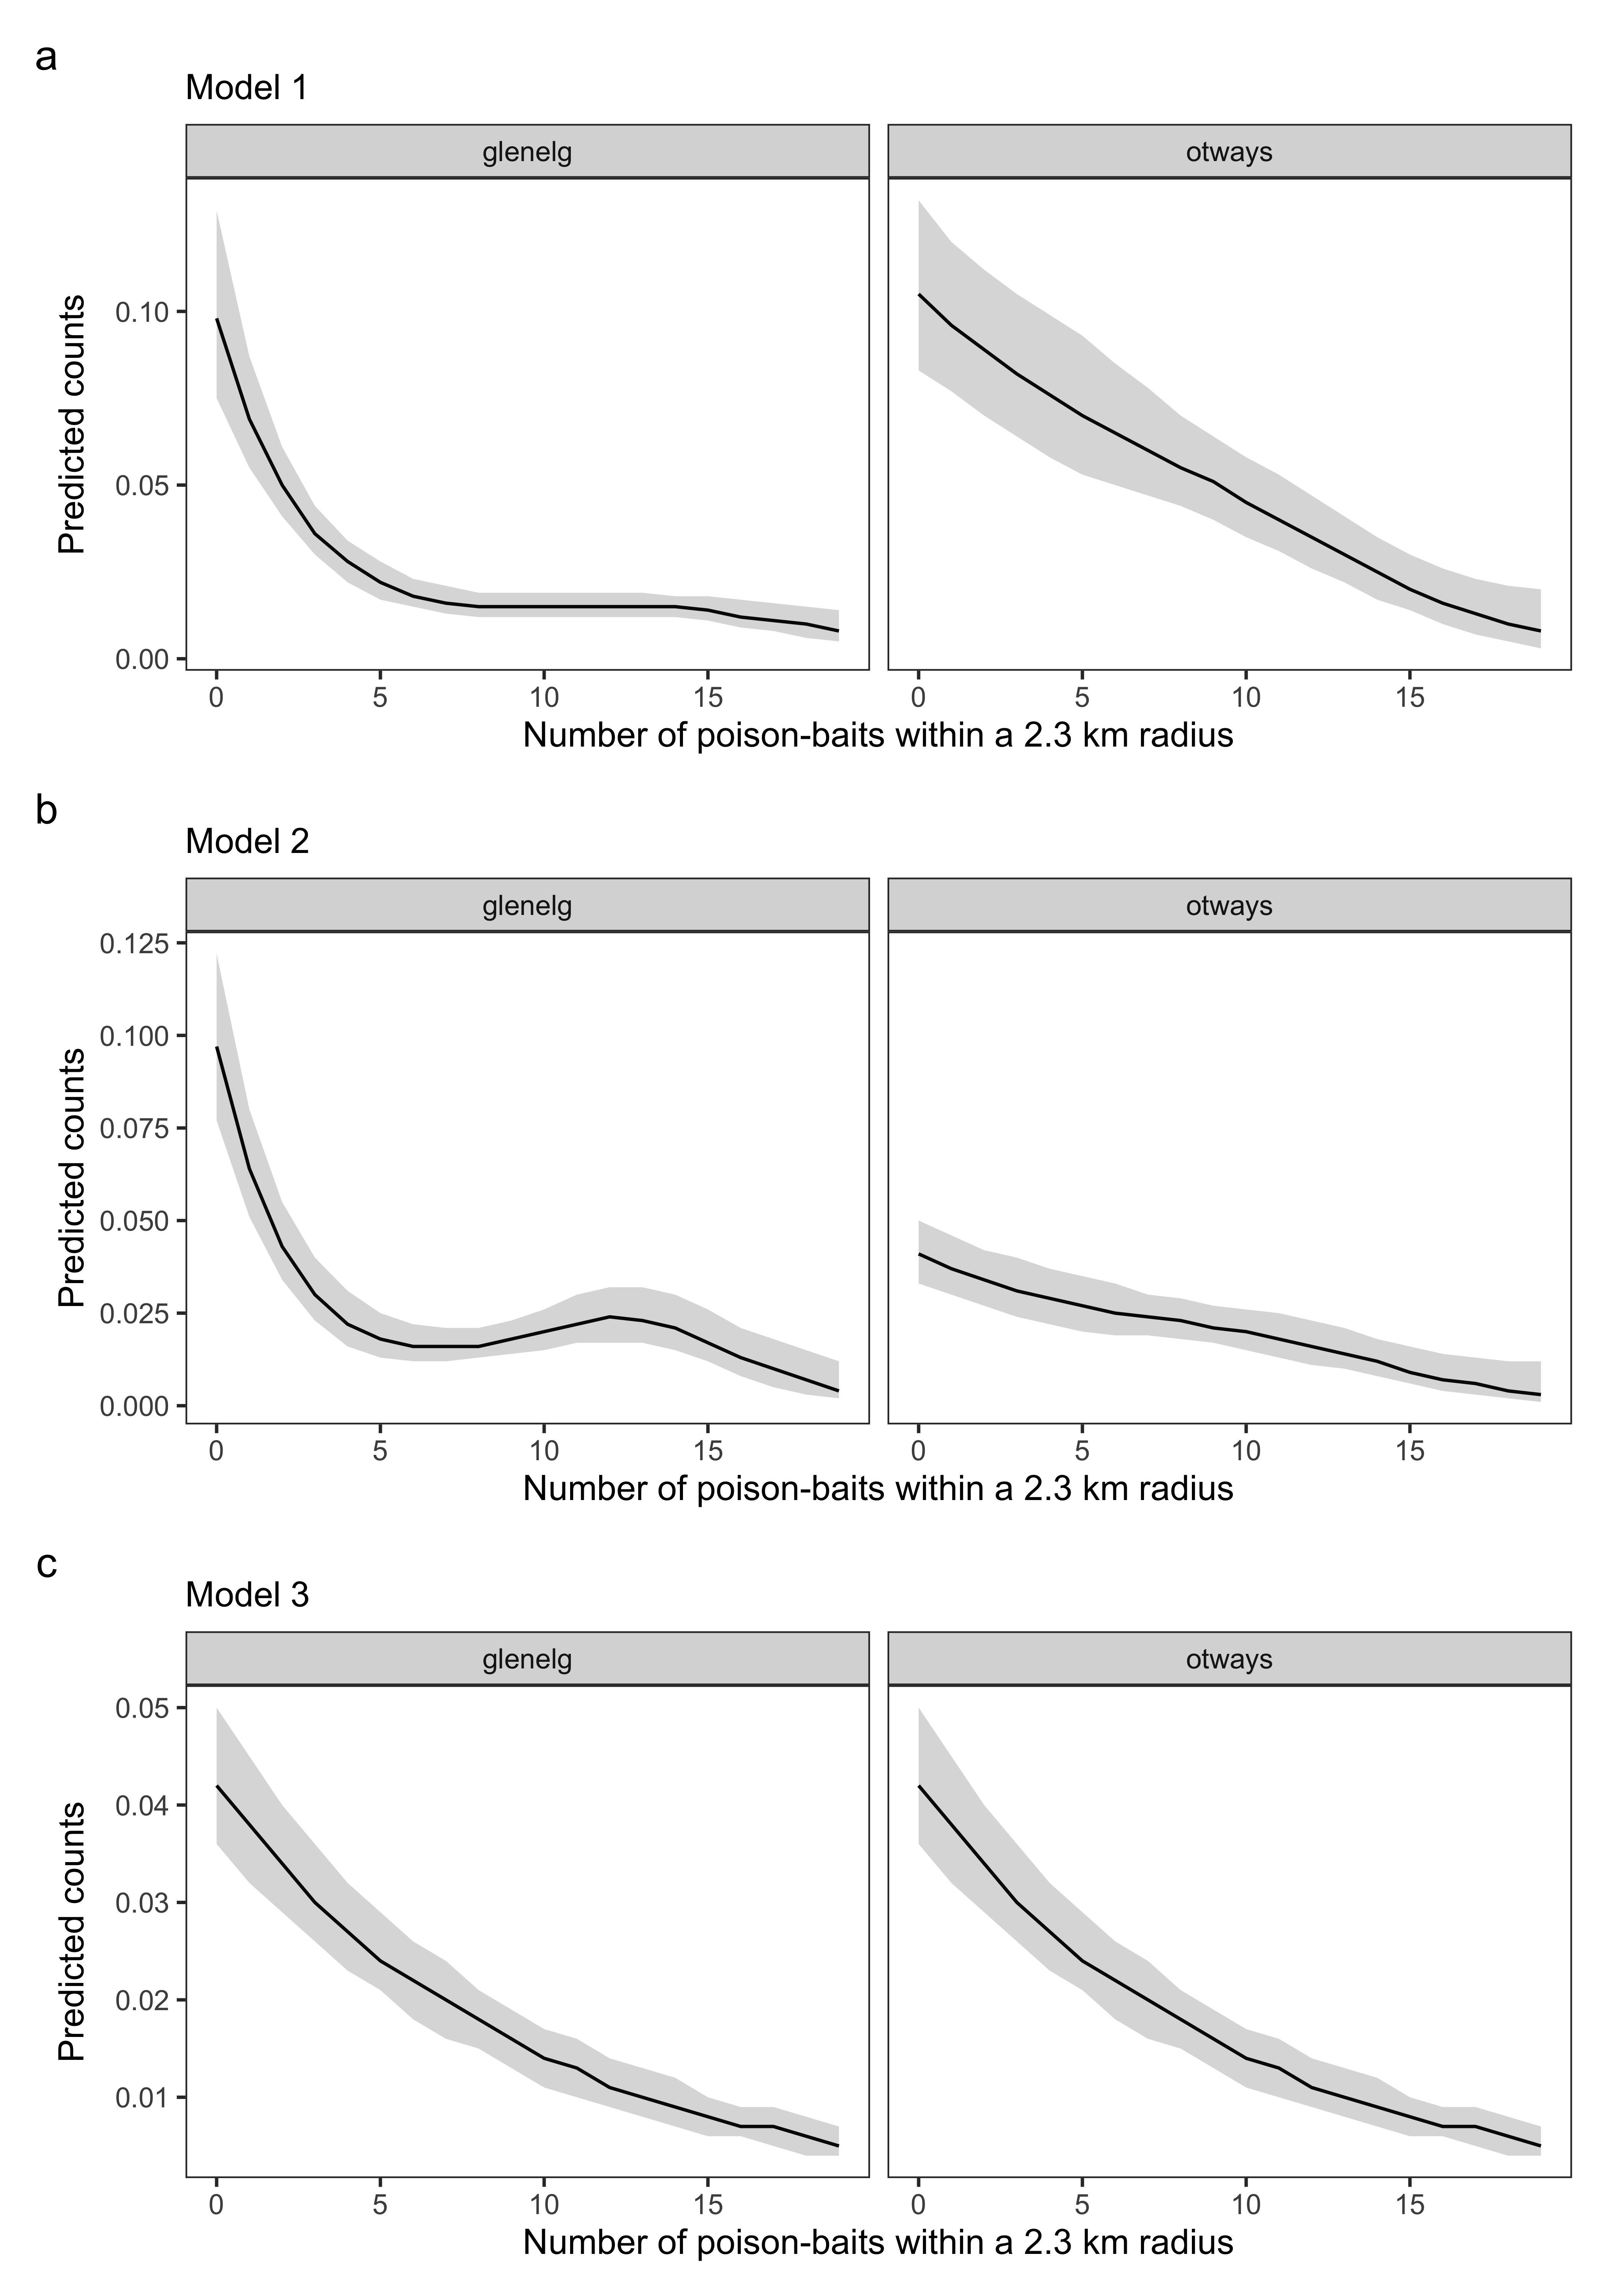
\includegraphics[width=0.8\linewidth]{../figs/foxbaiting_effects} 

}

\caption{Effects of 1080 poison-bait density on the spatial activity of red foxes \textit{Vulpes vulpes}, derived from each model (model 1: spatial, model 2: vegetation group / human footprint, model 3: habitat type). Shaded areas indicate 95\% confidence intervals.}\label{fig:fox-baits}
\end{figure}

\begin{figure}

{\centering 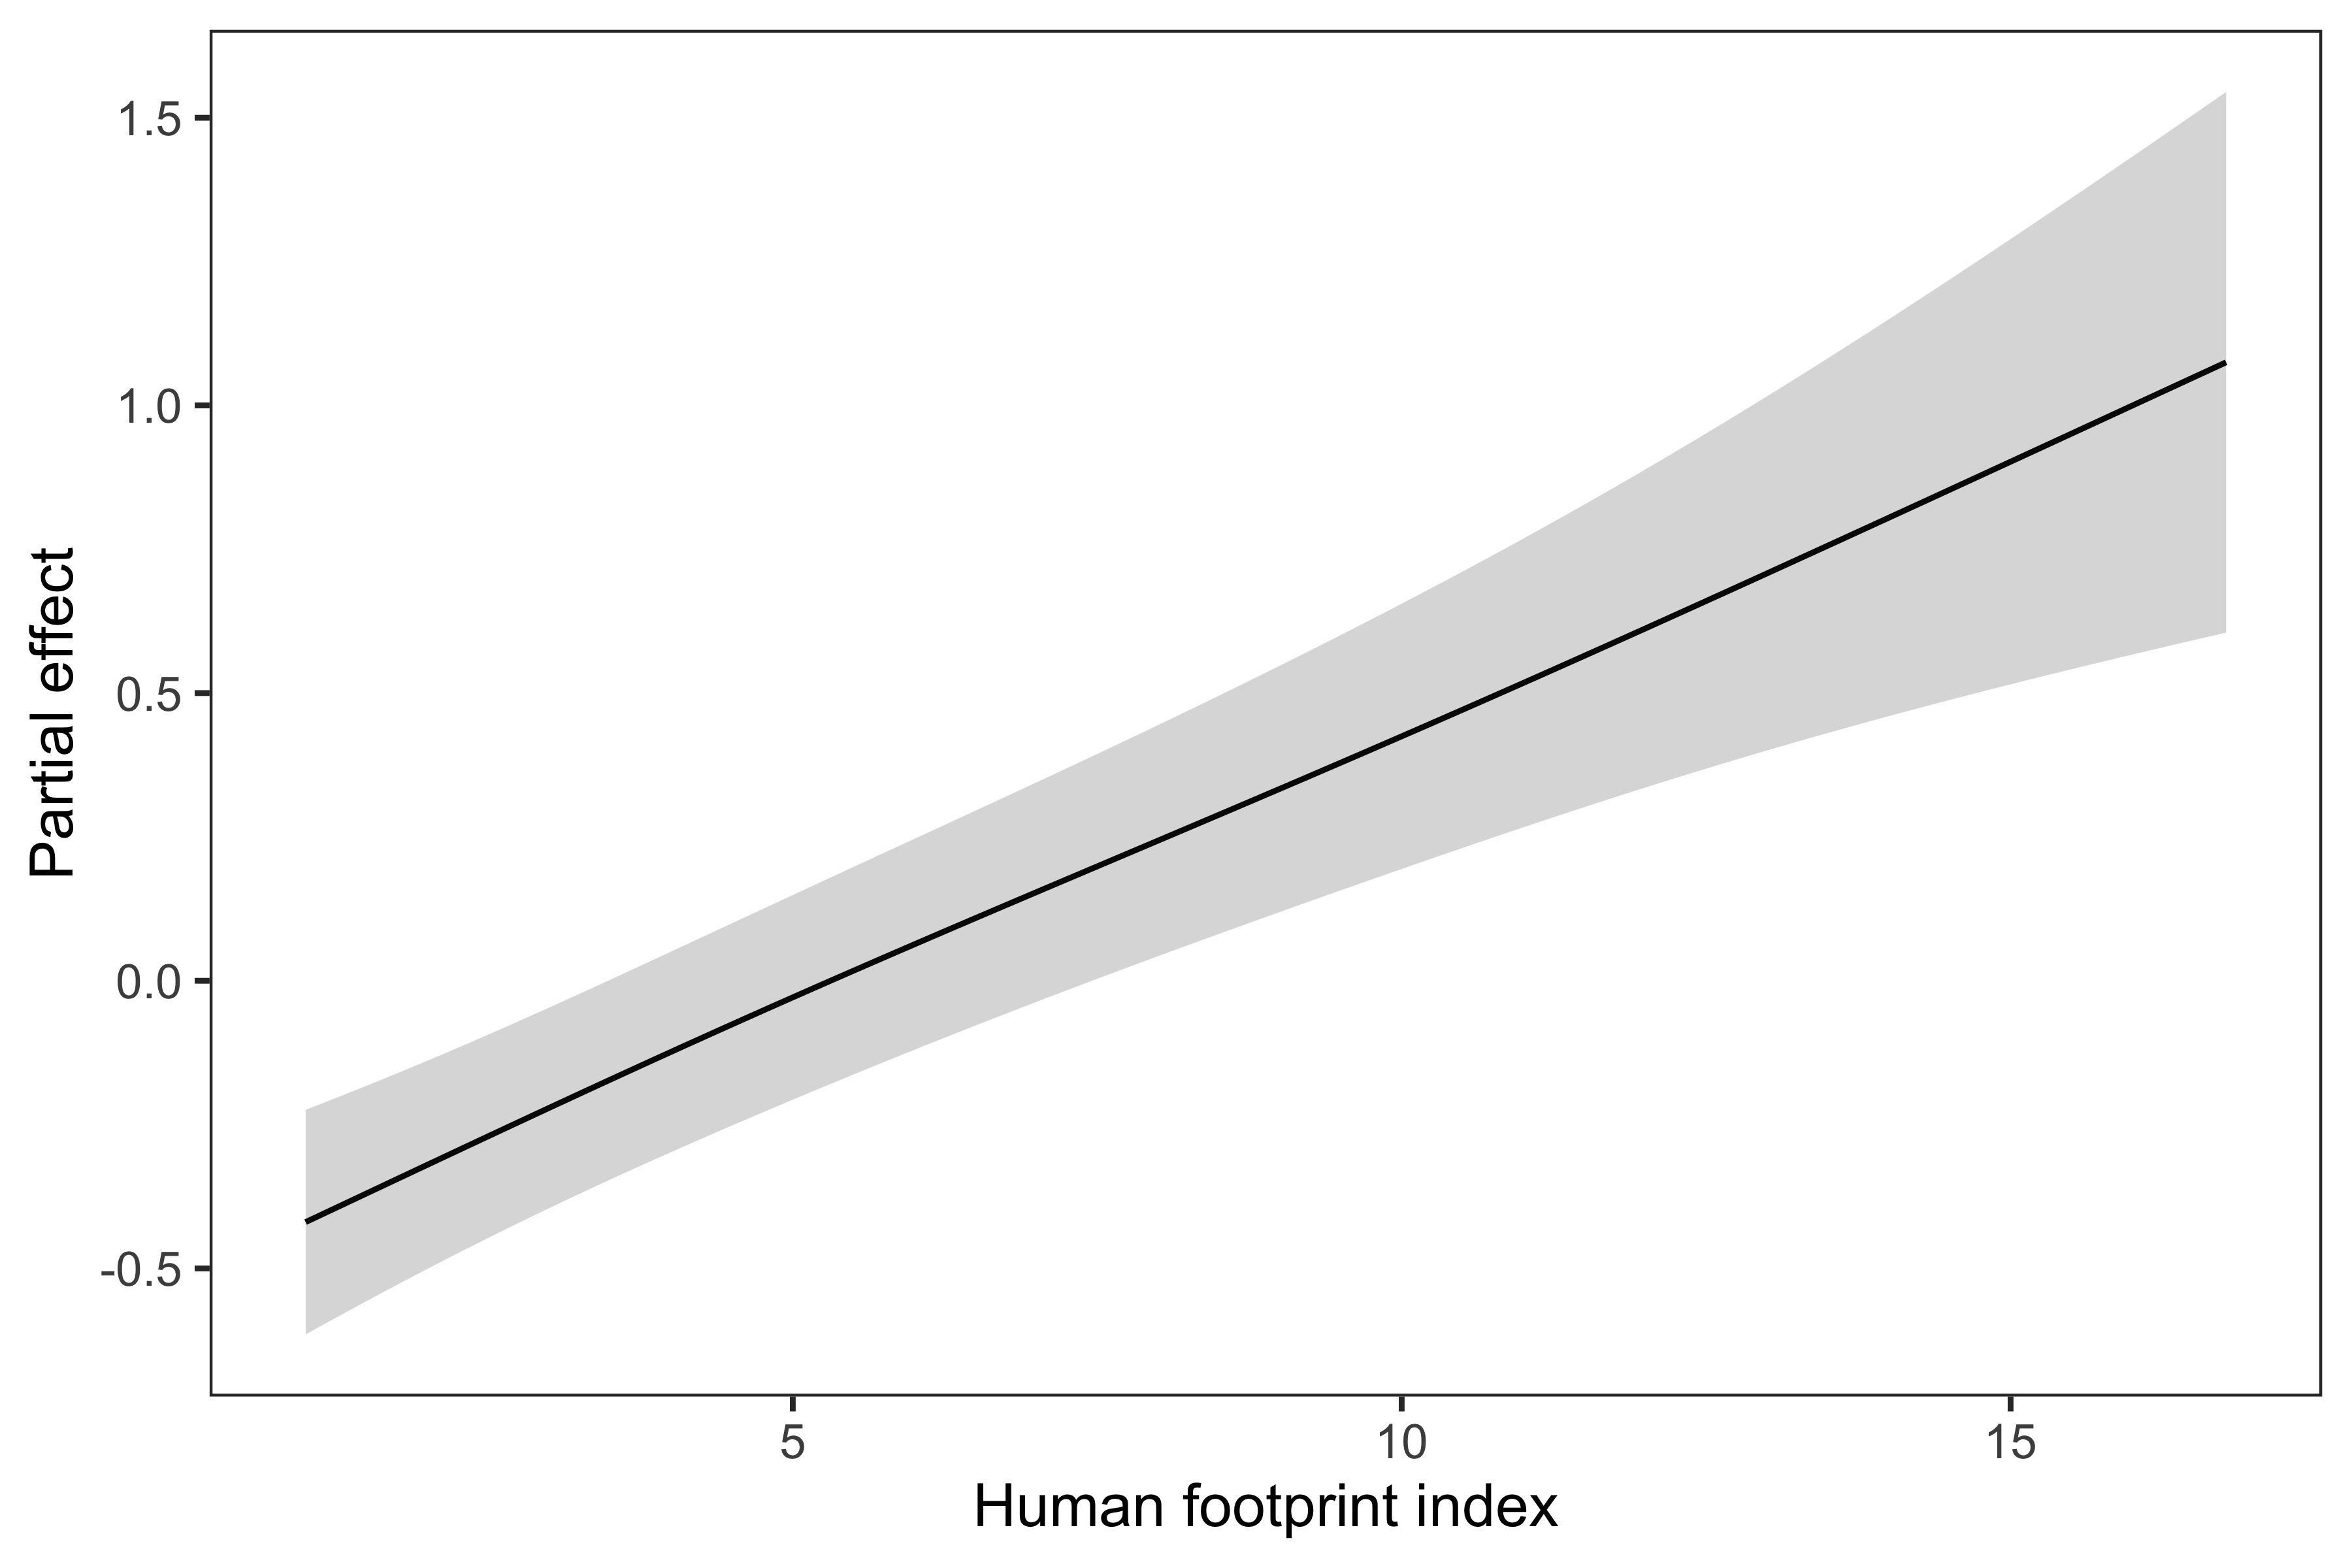
\includegraphics[width=0.8\linewidth]{../figs/fox_hfi} 

}

\caption{Effects human footprint index on the spatial activity of red foxes \textit{Vulpes vulpes}. (model 2). The interaction effect of human foot print and fox diel activity pattern was removed from this model. Both the marginal and interactive effect of human footprint was removed for feral cats \textit{Felis catus}). Shaded areas indicate 95\% confidence intervals.}\label{fig:fox-hfi}
\end{figure}


\end{document}
